%%%%%%%%%%%%%%%%%%%%%%%%%%%%%%%%%%%%%%%%%%%%%%%%%%%%%%%%%%%%%%%%%%%%%%%%%%%%%%%%%%%%%%
% Template per relazioni per l'Università di Firenze
% Autori: Iacopo Masi e Marco Meoni (riadattata da Gianluca Gorni)  
% Usare una versione di LaTeX con sillabazione italiana 
%%%%%%%%%%%%%%%%%%%%%%%%%%%%%%%%%%%%%%%%%%%%%%%%%%%%%%%%%%%%%%%%%%%%%%%%%%%%%%%%%%%%%%

\documentclass[12pt,a4paper,oneside,italian]{book}

% Usare "oneside" invece di "twoside"
% nelle bozze, per risparmiare carta:
% "twoside" produce diverse pagine bianche
% alla fine dei capitoli.

                    %%%%%%%%%%%%%%%%%%%%%%%%%%%%%%%%
                    %         inputenc             %
                    %  Usare l'opzione "latin1"    %
		    %  oppure "utf8"   		   %
                    %  se si vogliono scrivere     %
%                   %  lettere accentate da        %
                    %  tastiera su Windows o Unix  %
                    %%%%%%%%%%%%%%%%%%%%%%%%%%%%%%%%
% \usepackage[utf8x]{inputenc}

\usepackage[utf8]{inputenc}
% \usepackage[latin1]{inputenc}
\usepackage{rotating}
\usepackage{fancyvrb}
\usepackage{verbatim}
       %%%%%%%%%%%%%%%%%%%%%%%%%%%%%%%%%%%%%%%%%%%%%%
       %                  babel                     %
       % Pacchetto tipico per una tesi in italiano. %
       %%%%%%%%%%%%%%%%%%%%%%%%%%%%%%%%%%%%%%%%%%%%%%


\usepackage[italian]{babel}

   %%%%%%%%%%%%%%%%%%%%%%%%%%%%%%%%%%%%%%%%%%%%%%%%%%%%%%%%%%%%
   % Se nella tesi si inseriscono dei passi in un'altra       %
   % lingua (inglese, per fissare le idee), si puo' istruire  %
   % il TeX di sillabare quella parte di testo con le regole  %
   % inglesi, invece che italiane. A questo scopo basta       %
   % scrivere                                                 %
   %                                                          %
   %    \usepackage[english,italian]{babel}                   %
   %                                                          %
   % al posto di \usepackage[italian]{babel},                 %
   % dopodiche la sillabazione sara' italiana fintanto che    %
   % non si incontra il comando \selectlanguage{english}.     %
   % Per tornare all'italiano si scrive                       %
   % \selectlanguage{italian}                                 %
   %%%%%%%%%%%%%%%%%%%%%%%%%%%%%%%%%%%%%%%%%%%%%%%%%%%%%%%%%%%%

\usepackage{unifitesi}

% \usepackage{graphicx} % gia' caricato da unifitesi
\graphicspath{{./figure/}}

% Per l'ipertesto:
% \usepackage{hyperref} % gia' caricato da unifitesi
\hypersetup{
  % pdfpagelayout=SinglePage, % default
  % pdfpagemode=UseOutlines, % default
  % bookmarksopen, % default
  % bookmarksopenlevel=2, % default;
  pdftitle=Relazione sull'elaborato video-tracker sviluppato per l'esame Analisi Immagini e Video,
  pdfauthor=Marco Meoni Nicola Martorana Iacopo Masi,
  pdfsubject=video tracking tramite kalman e condensation,
  pdfkeywords=relazione Ingegneria Informatica Firenze video tracker videotracker opencv kalman condensation,} % Queste informazioni non vengono stampate, ma sono conservate nel documento pdf. Sono consultabili col menu "File>Document Properites>Description". Vengono buone a scopi archivistici.
%%%%%%%%%%%%%%%%%%%%%%%%%%%%%%%%%%%%%%%%%%%%%%%%%%%%%%%%%%%%

       %%%%%%%%%%%%%%%%%%%%%%%%%%%%%%%%%%%%%%%%%%%%%%%%
       % Pacchetti tipici per una tesi di matematica  %
       %%%%%%%%%%%%%%%%%%%%%%%%%%%%%%%%%%%%%%%%%%%%%%%%

\usepackage{amsmath,amsfonts,amssymb,amsthm}
\usepackage{latexsym}
%\usepackage{vertbars}
\usepackage{changebar}

%%%%%%%%%%%%%%%%%%%%%%%%%%%%%%%%%%%%%%%%%%%%%%%%%%%%%%%
%                    graphicx                         %
%                                                     %
%   Uno dei pacchetti per l'inserzione di figure      %
%   in formato eps e` "graphicx". Ce ne sono diversi  %
%   altri da cui scegliere.                           %
%                                                     %
%   Esempio di uso: avendo un file di nome            %
%   figura1.eps questa si inserisce nella tesi        %
%   col comando                                       %
%                                                     %
%        \begin{figure}[ht]                           %
%        \begin{center}                               %
%        \includegraphics{figura1.eps}                %
%        \caption[nome breve]{nome lungo}             %
%        \end{center}                                 %
%        \end{figure}                                 %
%                                                     %
%   Il "nome breve" e` quello che apparira`           %
%   nell'indice delle figure ed e' opzionale.         %
%   Il "nome lungo" e' quello che appare              %
%   sotto la figura.                                  %
%   (Ci sono opzioni per scalare, spostare, ruotare   %
%   le figure).                                       %
%   Con \graphicspath{{./figure/}} si dice            %
%   al LaTeX di cercare le figure nella cartella      %
%   "figure" situata allo stesso livello di           %
%   questo documento                                  %
%                                                     %
%%%%%%%%%%%%%%%%%%%%%%%%%%%%%%%%%%%%%%%%%%%%%%%%%%%%%%%

\linespread{1.3}
 %%%%%%%%%%%%%%%%%%%%%%%%%%%%%%%%%%%%%%%%%%%%%%%%%%
 % usate linesprea 1.6 per avere interlinea doppio%
 %%%%%%%%%%%%%%%%%%%%%%%%%%%%%%%%%%%%%%%%%%%%%%%%%%

  %%%%%%%%%%%%%%%%%%%%%%%%%%%%%%%%%%%%%%%%%%%
   %  Esempi di macro definite dall'utente.  %
   %  Le prime definiscono dei comandi per   %
   %  scrivere i caratteri speciali per      %
   %  gli insiemi numerici fondamentali      %
   %  (naturali, interi, razionali, reali,   %
   %  complessi                              %
   %%%%%%%%%%%%%%%%%%%%%%%%%%%%%%%%%%%%%%%%%%%

\newcommand{\N}{\mathbb{N}}
\newcommand{\Z}{\mathbb{Z}}
\newcommand{\Q}{\mathbb{Q}}
\newcommand{\R}{\mathbb{R}}
\newcommand{\C}{\mathbb{C}}


   %%%%%%%%%%%%%%%%%%%%%%%%%%%%%%%%%%%%%%%%%%%%
   %  Delle macro che definiscono operatori   %
   %  non predefiniti in LaTeX. Ogni utente   %
   %  aggiunge quelle che servono. Questi     %
   %  sono solo esempi arbitrari.             %
   %%%%%%%%%%%%%%%%%%%%%%%%%%%%%%%%%%%%%%%%%%%%

\DeclareMathOperator{\traccia}{tr}
\DeclareMathOperator{\sen}{sen}
\DeclareMathOperator{\arcsen}{arcsen}
\DeclareMathOperator*{\maxlim}{max\,lim}
\DeclareMathOperator*{\minlim}{min\,lim}
\DeclareMathOperator*{\deepinf}{\phantom{\makebox[0pt]{p}}inf}

    %%%%%%%%%%%%%%%%%%%%%%%%%%%%%%%%%%%%%%%%%%%%
    % Esempi di macro piu` elaborate,          %
    % contenenti degli argomenti.              %
    % Compongono gli indici delle sommatorie   %
    % e delle produttorie in modo diverso      %
    % da quello standard del TeX. Dovrebbero   %
    % funzionare bene quando gli estremi della %
    % sommatoria sono piccoli. Chi volesse     %
    % usarle estesamente farebbe bene a        %
    % lavorarci sopra.                         %
    %%%%%%%%%%%%%%%%%%%%%%%%%%%%%%%%%%%%%%%%%%%%

\newcommand{\varsum}[3]{\sum_{#2}^{#3}\!
   {\vphantom{\sum}}_{#1}\;}
\newcommand{\varprod}[3]{\sum_{#2}^{#3}\!
   {\vphantom{\sum}}_{#1}\;}

  %%%%%%%%%%%%%%%%%%%%%%%%%%%%%%%%%%%%%%%%%%%%%%%%%%%%%%%
  %          Numerazione delle formule                  %
  % Se non specificato altrimenti, il LaTeX numera le   %
  % formule come (capitolo.formula) (per esempio (2.5)  %
  % e` la quinta formula del secondo capitolo).         %
  % Con le istruzioni seguenti invece la numerazione    %
  % diventa (capitolo.sezione.formula) (per esempio     %
  % (3.2.6) e` la sesta formula della seconda sezione   %
  % del terzo capitolo):                                %
  %%%%%%%%%%%%%%%%%%%%%%%%%%%%%%%%%%%%%%%%%%%%%%%%%%%%%%%

\makeatletter
\@addtoreset{equation}{section}
\makeatother
\renewcommand{\theequation}%
  {\thesection.\arabic{equation}}


              %%%%%%%%%%%%%%%%%%%%%%%%%%
              % Stile degli enunciati  %
              %%%%%%%%%%%%%%%%%%%%%%%%%%

%%%%%%%%%%%%%%%%%%%%%%%%%%%%%%%%%%%%%%%%%%%%%%%%%%%%%%%%%%%
% Con le dichiarazioni seguenti                           %
% teoremi, definizioni, proposizioni, lemmi e corollari   %
% vengono numerati capitolo per capitolo e con un         %
% contatore unico per tutti (per esempio, se subito dopo  %
% il Teorema 2.1 c'e' una definizione, questa sara'       %
% Definizione 2.2)                                        %
%%%%%%%%%%%%%%%%%%%%%%%%%%%%%%%%%%%%%%%%%%%%%%%%%%%%%%%%%%%

\theoremstyle{plain}
\newtheorem{teorema}{Teorema}[chapter]
\newtheorem{proposizione}[teorema]{Proposizione}
\newtheorem{lemma}[teorema]{Lemma}
\newtheorem{corollario}[teorema]{Corollario}

\theoremstyle{definition}
\newtheorem{definizione}[teorema]{Definizione}
\newtheorem{esempio}[teorema]{Esempio}

\theoremstyle{remark}
\newtheorem{osservazione}[teorema]{Osservazione}

  %%%%%%%%%%%%%%%%%%%%%%%%%%%%%%%%%%%%%%%%%%%%%%%%%%%%%%%%
  % I comandi si usano cosi`:                            %
  %                                                      %
  %   \begin{teorema}[di Pitagora]                       %
  %   La somma dei quadrati ecc.                         %
  %   \end{teorema}                                      %
  %                                                      %
  % Le parole "di Pitagora" fra parentesi quadre         %
  % sono facoltative. Non bisogna inserire               %
  % manualmente degli spazi prima e dopo gli enunciati,  %
  % perche' e` automatico!                               %
  %%%%%%%%%%%%%%%%%%%%%%%%%%%%%%%%%%%%%%%%%%%%%%%%%%%%%%%%


  %%%%%%%%%%%%%%%%%%%%%%%%%%%%%%%%%%%%%%%%%%%%%%%%%%%%%%%%%%%%%%
  % Il pacchetto amsthm definisce anche l'ambiente "proof"     %
  % per le dimostrazioni.                                      %
  % Esempio di uso:                                            %
  %                                                            %
  %   \begin{proof}                                            %
  %   Sia $X$ un insieme ecc.                                  %
  %   \end{proof}                                              %
  %                                                            %
  %%%%%%%%%%%%%%%%%%%%%%%%%%%%%%%%%%%%%%%%%%%%%%%%%%%%%%%%%%%%%%

       %%%%%%%%%%%%%%%%%%%%%%%%%%%%%%%%%%%%%%%%%%%%%%%%%%%%%%%
       %                   makeidx                           %
       %                                                     %
       % Pacchetto per la generazione automatica dell'indice %
       % analitico. Per esempio, se vogliamo che la parola   %
       % "analitico" venga indicizzata nella frase           %
       %                                                     %
       %    "un metodo analitico di soluzione"               %
       %                                                     %
       % bisogna scrivere                                    %
       %                                                     %
       %    "un metodo analitico\index{analitico} di         %
       %              soluzione".                            %
       %                                                     %
       % Compilando il file, il LaTeX produrra' un file      %
       % ausiliario che termina con ".idx". Bisogna far      %
       % processare questo file idx dal programma            %
       % ausiliario "bibtex", che produrra' a sua volta un   %
       % altro file ancora. Dare infine un'ultima passata    %
       % col LaTeX. Si puo' tranquillamente lasciare         %
       % la compilazione dell'indice verso la fine della     %
       % stesura del lavoro, quando tutto e' ormai quasi     %
       % definitivo.                                         %
       %                                                     %
       %%%%%%%%%%%%%%%%%%%%%%%%%%%%%%%%%%%%%%%%%%%%%%%%%%%%%%%

\usepackage{makeidx}
\usepackage{array}
\usepackage{tocbibind}
\usepackage{listings}
\usepackage{color}
\makeindex

% Ridefiniamo la riga di testa delle pagine:
\usepackage{fancyhdr}
\pagestyle{fancy}
\renewcommand{\chaptermark}[1]{\markboth{#1}{}}
\renewcommand{\sectionmark}[1]{\markright{\thesection\ #1}}
\fancyhf{}
\fancyhead[LE,RO]{\thepage}
\fancyhead[LO]{\rightmark}
\fancyhead[RE]{\bfseries\leftmark}
\renewcommand{\headrulewidth}{0.1pt}
\renewcommand{\footrulewidth}{0pt}
\headsep=50pt


               %%%%%%%%%%%%%%%%%%%%%%%%%%%%%%%%%%%%%%
               %  Informazioni generali sulla Tesi  %
               %    da usare nell'intestazione      %
               %%%%%%%%%%%%%%%%%%%%%%%%%%%%%%%%%%%%%%
%\titolo{Analisi del Software Libero e del software OpenSource con particolare attenzione all'interoperabilità e alla portabilità}
%\titolo{Analisi tecnico/giuridica del Copyleft con particolare attenzione all'interoperabilità e portabilità.}
\titolo{Comparazione di Kalman e ConDensation in video-tracking}
%\titolo{Analisi tecnico-giuridica dell'interoperabilità e della portabilità nello sviluppo di Software Libero e di software OpenSource}

 \laureando{MMM Team}
  \annoaccademico{2006-2007}
 \facolta{Ingegneria} % (default)
  \corsodilaurea{Ingegneria Informatica} % per la laurea vecchio ordinamento
% \corsodilaureatriennale{Informatica}
% \corsodilaureaspecialistica{Ingegneria}
  \relatore[Prof.]{Pietro Pala}
  \correlatore[Ing.]{Walter Nunziati}
  \correlatoredue[Ing.]{Andy Bagdanov}
  
  %\dedica{\textit{``Baby don't cry\\make it funky''} \\Zucchero} % (facoltativo)
% 
   %%%                                    %        %%    %%
  %   %                                   %         %     %
  %      %%%  % %%  %%%%   %%%         %%%%  %%%    %     %    %%%%
  %     %   % %%  % %   % %   %       %   % %   %   %     %   %   %
  %     %   % %     %   % %   %       %   % %%%%%   %     %   %   %
  %   % %   % %     %   % %   %       %   % %       %     %   %  %%
   %%%   %%%  %     %%%%   %%%         %%%%  %%%%  %%%   %%%   %% %
                    %
                    %


                          %%%%%               %
                            %
                            %    %%%   %%%%  %%
                            %   %   % %       %
                            %   %%%%%  %%%    %
                            %   %         %   %
                            %    %%%% %%%%   %%%


 \begin{document}

         %%%%%%%%%%%%%%%%%%%%%%%%%%%%%%%%%%%%%%%%%%%%%%%%%
         %            Intestazione                       %
         %                                               %
         % Per l'intestazione completa bisogna           %
         % essersi procurati il file "firenze.eps". %
         %%%%%%%%%%%%%%%%%%%%%%%%%%%%%%%%%%%%%%%%%%%%%%%%%

\frontmatter
\maketitle


\tableofcontents
\listoffigures
%\lstlistoflistings


%\lstset{language=C++} 

\lstset{
%basicstyle=\small,
%numbers=none,
%numberstyle=\tiny,
%stepnumber=1,
%numbersep=2pt, 
%frame=TB,
%framesep=5pt,
%  xleftmargin=0.3cm,
basicstyle=\ttfamily,
keywordstyle=\color{blue}\ttfamily,
ndkeywordstyle=\color{yellow}\ttfamily,
identifierstyle=\ttfamily,
commentstyle=\color{red}\ttfamily,
stringstyle=\color{black}\ttfamily,
%directivestyle=\color{magenta}\ttfamily
} 


\section{Introduzione}
Questa relazione descrive lo studio effettuato, i metodi utilizzati ed i risultati raggiunti per la realizzazione dell'elaborato relativo al corso di Analisi delle immagini e dei video, appartenente al corso di laurea specialistica in Ingegneria Informatica di Firenze, tenuto dal Prof. Pietro Pala.

L'elaborato si è incentrato sullo studio di due algoritmi di \textit{tracking} video, il filtro di Kalman ed il ConDensation, iniziando con l'approfondimento delle rispettive basi teoriche per poi passare all'implementazione di entrambi, finalizzata all'ottenimento di risultati comparativi, che sono stati catalogati ed interpretati. Lo sviluppo dell'elaborato è stato coordinato all'interno del \textit{Media Integration and Communication Center}\footnote{MICC, http://www.micc.unifi.it/} in particolare dall'Ing. Walter Nunziati e dall'Ing. Andrew D. Bagdanov, ai quali va un particolare ringraziamento per l'attenzione che hanno riposto in questo lavoro.
\begin{figure}[hb]
\centering
	
\includegraphics[scale=0.6]{micc.png}
\caption{\textit{Media Integration and Communication Centre, Firenze}\label{fig:micc}}
\end{figure}

L'implementazione del software che ha fornito i risultati comparativi è stata effettuata nel linguaggio di programmazione C++ tramite le librerie per il computer vision OpenCV\footnote{Open Source Computer Vision Library http://www.intel.com/technology/computing/opencv/}, sviluppate internamente ad Intel, ma rese pubblicamente fruibili ed utilizzabili tramite una licenza \textit{GPL-compatibile}; lo sviluppo del codice è stato effettuato sotto controllo di versione Subversion (SVN), in hosting presso Google Code\footnote{http://code.google.com/p/video-tracker/}. Il software è stato reso pubblico sotto licenza libera GNU GPL\footnote{GNU General Public License http://www.gnu.org/licenses/gpl.html}.

Grazie al sistema di controllo di versione è stato possibile sviluppare il software contemporaneamente sia sotto architettura Unix (nello specifico diverse distribuzioni di GNU/Linux) che sotto architettura Microsoft Windows, risultando così pienamente compatibile con entrambe.

Con questa relazione ci si prefigge l'obiettivo di ripercorrere il cammino fatto nello sviluppo dell'elaborato, iniziando nel primo capitolo con una introduzione ai due metodi di \textit{tracking}, con un breve approfondimento delle rispettive basi matematiche per poi concludere focalizzando l'attenzione sulla specifica implementazione del modello utilizzato.

La descrizione passerà nel secondo capitolo ad affrontare lo sviluppo del software che ha reso possibile lo sviluppo della comparazione, approfondendo i punti fondamentali delle librerie utilizzate per andare poi ad analizzare dettagliatamente il \textit{control-flow} del programma. 

L'ultima sezione sarà invece dedicata allo studio dei risultati ottenuti, e fornirà i risultati più importanti di tutta la serie di esperimenti che sono stati compiuti con il software ottenuto, riportandone grafici comparativi e schermate di esecuzione.

%Rapida descrizione dell'elaborato e di come si articola la relazione, motivazioni della ricerca ecc...
\mainmatter
     %%%%%%%%%%%%%%%%%%%%
     %                                                   %
     %  capitolo1.tex   %
     %                  %
     %%%%%%%%%%%%%%%%%%%%

\section{Esperimenti}\label{sec:esperimenti}

Il software prodotto è stato testato su molteplici video, tra i quali ne sono stati selezionati tre che si distinguevano per le condizioni di esecuzione, in particolare stimolando caratteristiche specifiche dei due algoritmi di tracking, in modo da efatizzarne i risultati. I tre filmati sono caratterizzati da una ripresa a camera fissa, con un singolo oggetto in movimento che può sia uscire dall'inquadratura che nascondersi dietro qualche ostacolo all'interno della scena (occlusione). 

In ognuno dei tre filmati i primi frames sono di solo sfondo, ovvero non compare alcun oggetto in moto; questa scelta è stata effettuata per facilitare l'applicazione del Background Subtraction.\\

Per ciascun video abbiamo osservato/confrontato il comportamento dei due filtri al variare di alcuni parametri quali:
\begin{itemize}
\item frequenza di campionamento (MOD)
\item covarianza relativa al rumore del processo studiato (Q) (stabilisce la tolleranza consentita alla predizione del filtro di Kalman)
\item numero di campioni utilizzati dal Condensation\\
\end{itemize}

I risultati prodotti per ciascuna prova sono rappresentati in due grafici:
\begin{itemize}
\item Il primo rappresenta per ogni campionamento:
\begin{itemize}
\item la posizione dell'oggetto
\item la posizione predetta dal filtro di Kalman
\item la posizione predetta dal Condensation
\end{itemize}
\item Il secondo rappresenta per ogni campionamento di quanto rispettivamente ciascuna predizione si discosta dalla posizione reale dell'oggetto.
\end{itemize}

Inoltre per ogni test viene dato il valore medio della distanza (in pixels) tra posizione predetta e posizione reale, sia per il filtro di Kalman \begin{math}(\bar \delta_K)\end{math} che per il Condensation \begin{math}(\bar \delta_C)\end{math}, oltre al valore della varianza media per il Condensation \begin{math}(\sigma_x,\sigma_y)\end{math}.


\newpage

\subsection{Video: movies12.mjpeg}\label{sec:video-occ}
\begin{itemize}
\item risoluzione: 640x480
\item fps: 25.00
\item durata: 50.4 s
\end{itemize}

\begin{figure}[hb]
\centering
	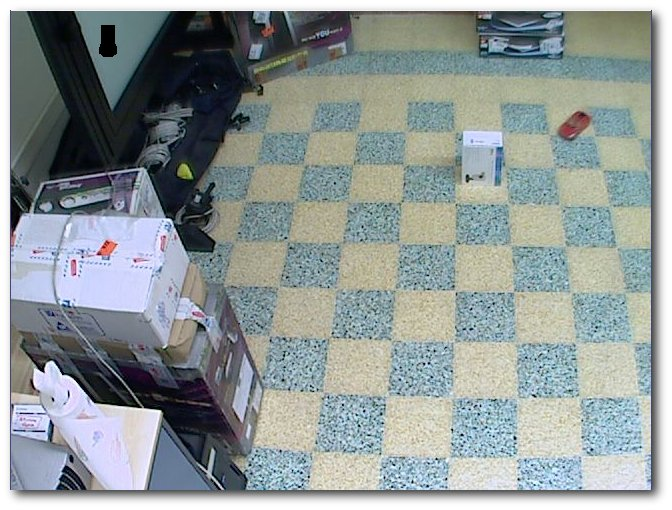
\includegraphics[scale=0.5]{movie12.jpg}
\caption{\textit{movie12 screenshot}}
\end{figure}

Si tratta di una ripresa trasversale dall'alto di un automobilina radiocomandata. In questa scena i punti di occlusione sono due: una scatola al centro della scena e un ostacolo sulla sinistra. La macchina non subisce repentine accelerazioni o decelerazioni, in generale ruota attorno alla scatola centrale e riamane nascosta dietro questa per un po'. L'automobilina non esce mai dalla scena.

%\begin{figure}[hb]
%\centering%
%	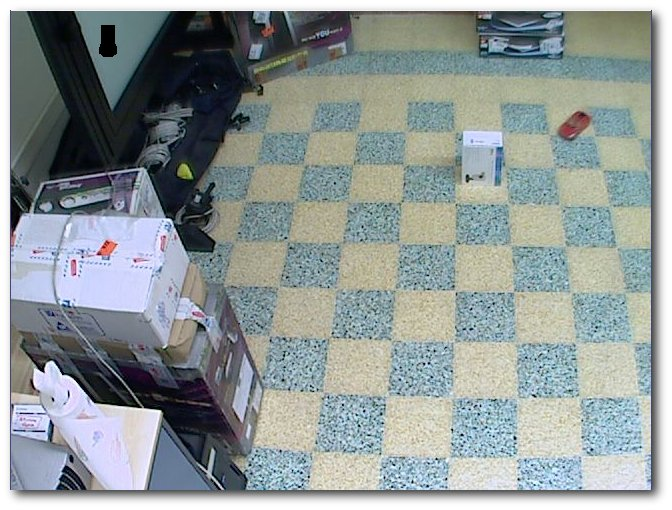
\includegraphics[scale=0.5]{movie12.jpg}
%\caption{\textit{movie12 screenshot}}
%\end{figure}
 
\newpage
\subsubsection{Test 1: MOD=3 , Q=1000, S=1000}

\begin{figure}[hb]
\centering
	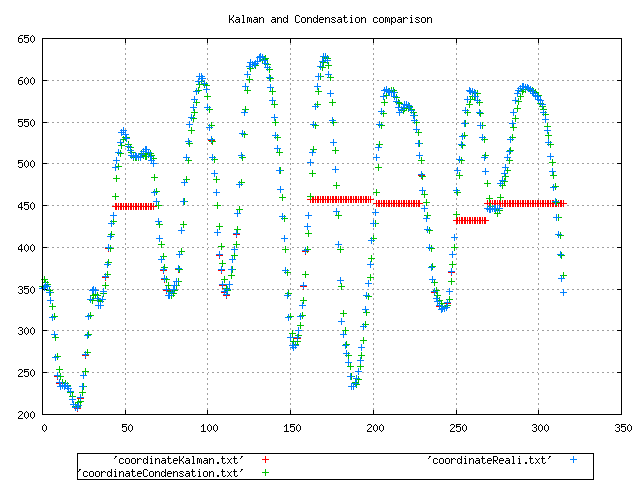
\includegraphics[scale=0.4]{../../esperimenti/movie12/mod_3-Q_1000-S_1000/plot.png}
\caption{\textit{Test 1: Tracciamento}}
\end{figure}

\begin{figure}[hb]
\centering
	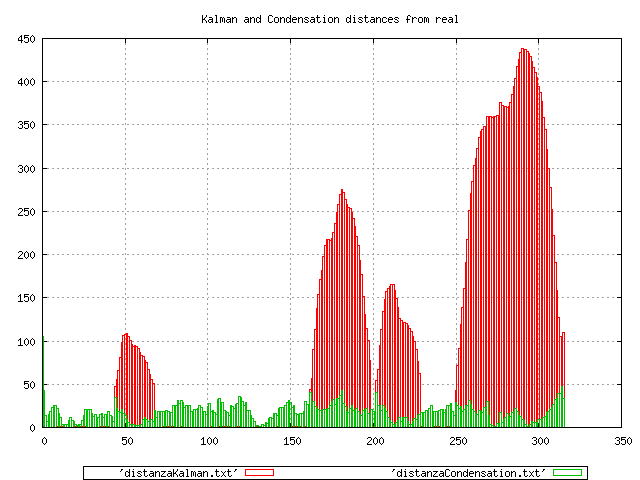
\includegraphics[scale=0.4]{../../esperimenti/movie12/mod_3-Q_1000-S_1000/plot-distances.png}
\caption{\textit{Test 1: Previsioni}}
\end{figure}

Statistiche:
\begin{itemize}
\item \begin{math} \bar \delta_K: 105 \end{math}
\item \begin{math} \bar \delta_C: 18 \end{math}
\item \begin{math}(\sigma_x,\sigma_y)\end{math}: (112,81)
\end{itemize}

Appare evidente che con queste impostazioni il filtro di Kalman non è in grado di mantenere traccia correttamente dell'oggetto, poichè più di una misurazione è persa a causa dell'occlusione. L'area di tolleranza per Kalman non è sufficiente. Tuttavia non appena l'oggetto ripassa vicino a dove Kalman si è fermato, questo ricomincia ad essere tracciato correttamente. Differentemente il Condenstaion non perde mai l'oggetto, ma la stima del moto è decisamente meno precisa.

\newpage

\subsubsection{Test 2: MOD=3, Q=2000, S=1000}

\begin{figure}[hb]
\centering
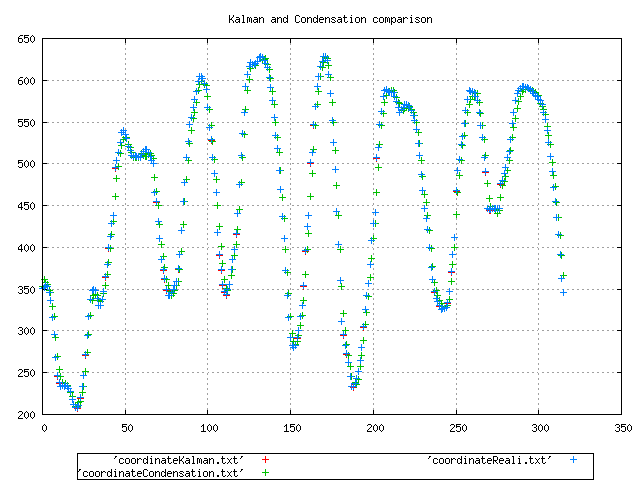
\includegraphics[scale=0.4]{../../esperimenti/movie12/mod_3-Q_2000-S_1000/plot.png}
\caption{\textit{Test 2: Tracciamento}}
\end{figure}

\begin{figure}[hb]
\centering
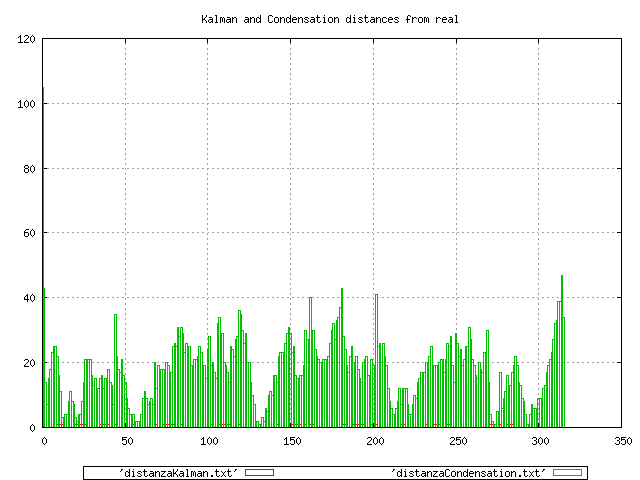
\includegraphics[scale=0.4]{../../esperimenti/movie12/mod_3-Q_2000-S_1000/plot-distances.png}
\caption{\textit{Test 2: Previsioni}}
\end{figure}

Statistiche:
\begin{itemize}
\item \begin{math} \bar \delta_K: 0 \end{math}
\item \begin{math} \bar \delta_C: 18 \end{math}
\item \begin{math}(\sigma_x,\sigma_y)\end{math}: (112,81)
\end{itemize}

Allargando l'area di confidenza per Kalman l'oggetto non viene mai perso e il tracciamento risulta pressochè perfetto. Il comportamrento in questo caso è evidentemente migliore del Condesation. Purtroppo un'area di confidenza troppo ampia potrebbe in alcune circostanze far perdere di validità al tracciamento. 

\newpage
\subsubsection{Test 3: MOD=3, Q=1000, S=5000}

\begin{figure}[hb]
\centering
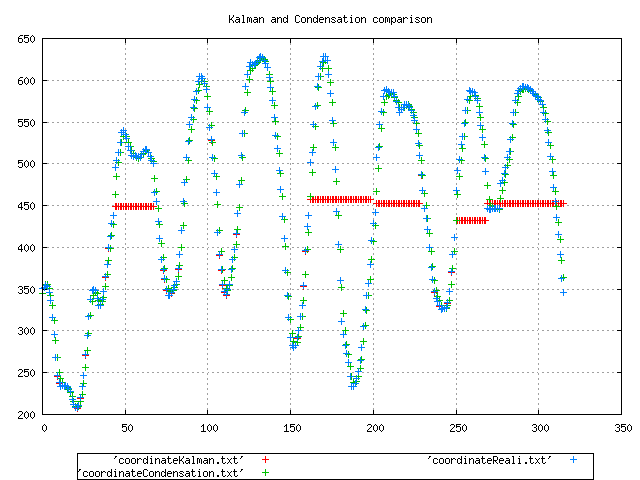
\includegraphics[scale=0.4]{../../esperimenti/movie12/mod_3-Q_1000-S_5000/plot.png}
\caption{\textit{Test 3: Tracciamento}}
\end{figure}

\begin{figure}[hb]
\centering
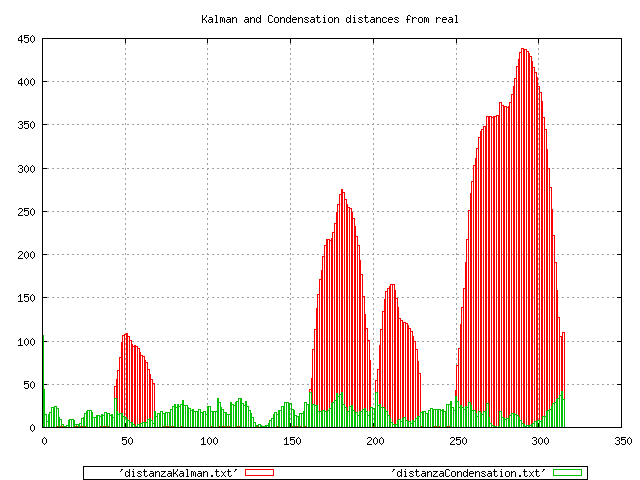
\includegraphics[scale=0.4]{../../esperimenti/movie12/mod_3-Q_1000-S_5000/plot-distances.png}
\caption{\textit{Test 3: Previsioni}}
\end{figure}

Statistiche:
\begin{itemize}
\item \begin{math} \bar \delta_K: 105 \end{math}
\item \begin{math} \bar \delta_C: 17 \end{math}
\item \begin{math}(\sigma_x,\sigma_y)\end{math}: (109,81)
\end{itemize}

Con questo test cominciamo a verificare il comportamento del Condensation alla variazione del numero di samples.
E' immediato osservare come aumentando il numero di samples da 1000 a 5000 questo non porti in media nessun significativo miglioramento.

\newpage
\subsubsection{Test 4: MOD=3, Q=1000, S=100}

\begin{figure}[hb]
\centering
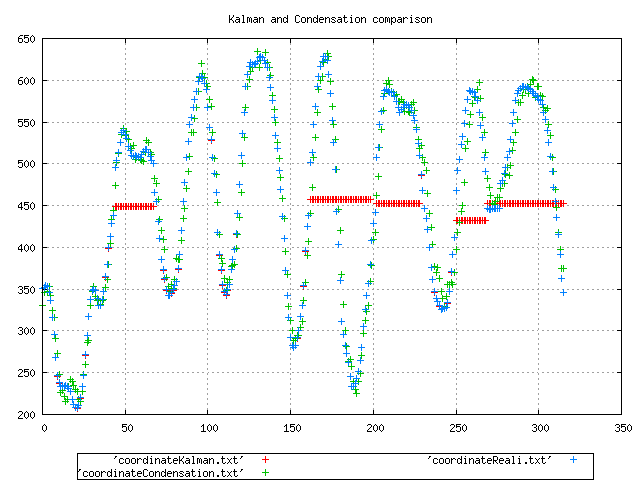
\includegraphics[scale=0.4]{../../esperimenti/movie12/mod_3-Q_1000-S_100/plot.png}
\caption{\textit{Test 4: Tracciamento}}
\end{figure}

\begin{figure}[hb]
\centering
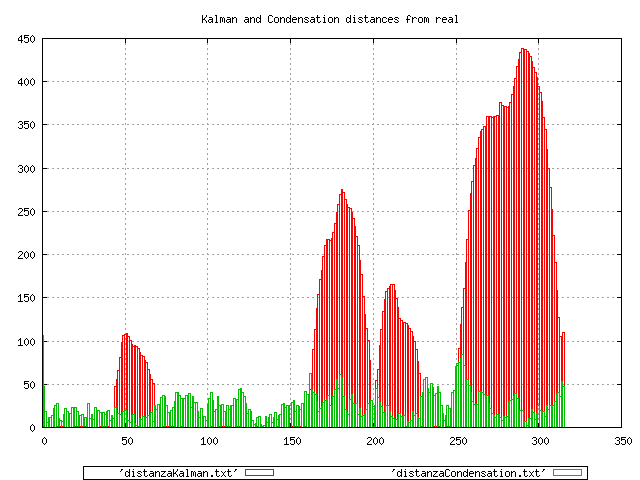
\includegraphics[scale=0.4]{../../esperimenti/movie12/mod_3-Q_1000-S_100/plot-distances.png}
\caption{\textit{Test 4: Previsioni}}
\end{figure}

Statistiche:
\begin{itemize}
\item \begin{math} \bar \delta_K: 105 \end{math}
\item \begin{math} \bar \delta_C: 24 \end{math}
\item \begin{math}(\sigma_x,\sigma_y)\end{math}: (140,92)
\end{itemize}


Di contro con questo test si nota come passando da 1000 a 100 samples invece il risultato sia notevolemente diverso. La stima del moto come si vede dal grafico è notevolemente peggiore nel secondo caso. 
Fortunatamente ha anche poco senso limitare così tanto il numero di samples, mentre un numero molto alto di samples per noi non comporta nessun particolare svantaggio. 

\newpage
\subsubsection{Test 5: MOD=3, Q=1000, S=10}

\begin{figure}[hb]
\centering
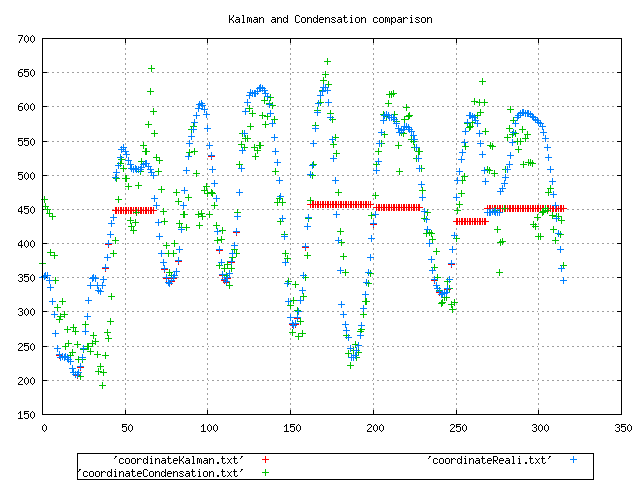
\includegraphics[scale=0.4]{../../esperimenti/movie12/mod_3-Q_1000-S_10/plot.png}
\caption{\textit{Test 5: Tracciamento}}
\end{figure}

\begin{figure}[hb]
\centering
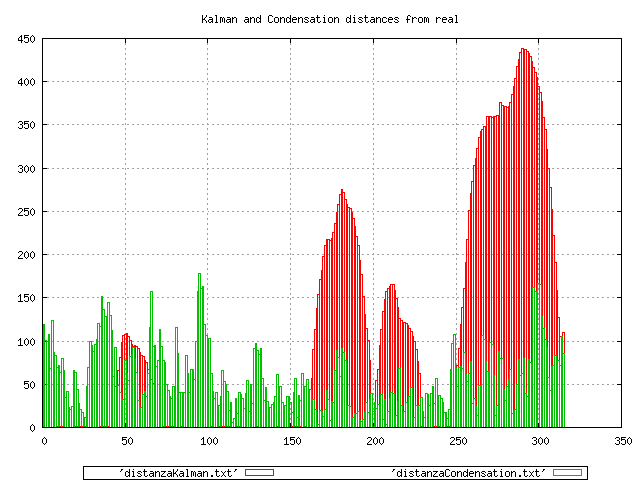
\includegraphics[scale=0.4]{../../esperimenti/movie12/mod_3-Q_1000-S_10/plot-distances.png}
\caption{\textit{Test 5: Previsioni}}
\end{figure}

Statistiche:
\begin{itemize}
\item \begin{math} \bar \delta_K: 105 \end{math}
\item \begin{math} \bar \delta_C: 55 \end{math}
\item \begin{math}(\sigma_x,\sigma_y)\end{math}: (195,112)
\end{itemize}


Abbiamo proseguito nel diminuire il numero di Samples per il Condensation passando a 10, il confronto tra il caso in cui i samples erano 1000 è autoesplicativo: il risultato è notevolemente peggiore. Come ci si poteva aspettare in condizioni estreme di lavoro le previsioni sono decisamente inattendibili.

\newpage
\subsection{Video: tappetonomod.avi}

\begin{itemize}
\item risoluzione: 320x240
\item fps: 10.00
\item durata: 60 s
\end{itemize}

Si tratta di una ripresa trasversale dall'alto. L'oggetto in movimento è un'automobilina radiocomandata che si muove su un'area delimitata da un tappeto. Il moto dell'automobilina subisce repentine accelerazioni e decelerazioni. Non ci sono oggetti occludenti, ma l'automobilina entra ed esce totalmente o parzialmente più di una volta dalla scena.

\begin{figure}[hb]
\centering
	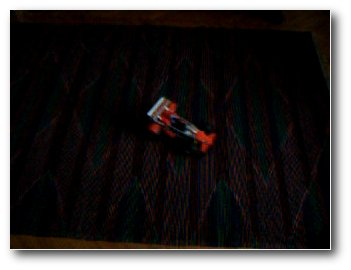
\includegraphics[scale=0.5]{tappeto_nomod.jpg}
\caption{\textit{tappeto-nomod screenshot}}
\end{figure}

\newpage
\subsubsection{Test 6: MOD=3, Q=1000, S=1000}

\begin{figure}[hb]
\centering
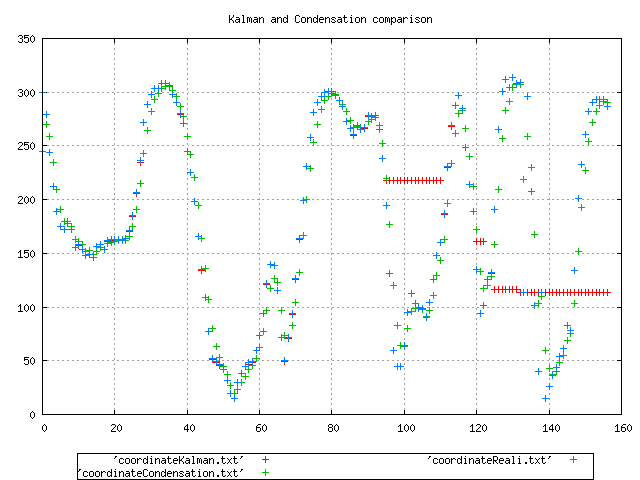
\includegraphics[scale=0.4]{../../esperimenti/tappeto_nozoom/mod_3-Q_1000-S_1000/plot.png}
\caption{\textit{Test 6: Tracciamento}}
\end{figure}

\begin{figure}[hb]
\centering
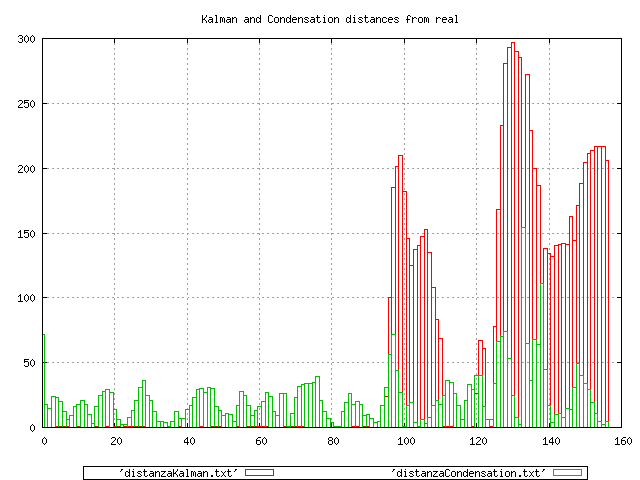
\includegraphics[scale=0.4]{../../esperimenti/tappeto_nozoom/mod_3-Q_1000-S_1000/plot-distances.png}
\caption{\textit{Test 6: Previsioni}}
\end{figure}

Statistiche:
\begin{itemize}
\item \begin{math} \bar \delta_K: 53 \end{math}
\item \begin{math} \bar \delta_C: 22 \end{math}
\item \begin{math}(\sigma_x,\sigma_y)\end{math}: (53,22)
\end{itemize}

La macchinina si sposta in modo molto rapido. Kalman si comporta in modo egregio fintanto che l'oggetto si trova nell'inquadratura e che l'accelerazione della macchina non è tale da far uscire l'oggetto dall'area di previsione. Il Condensation mantiene un buon comportamento anche se mai perfetto.

\newpage
\subsubsection{Test 7: MOD=5, Q=1000, S=1000}

\begin{figure}[hb]
\centering
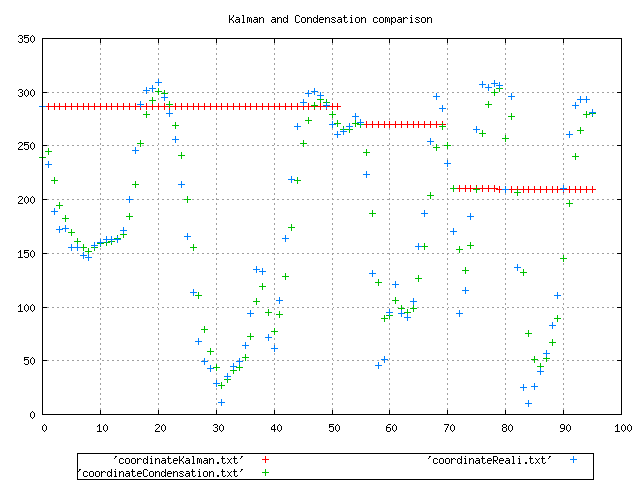
\includegraphics[scale=0.4]{../../esperimenti/tappeto_nozoom/mod_5-Q_1000-S_1000/plot.png}
\caption{\textit{Test 7: Tracciamento}}
\end{figure}

\begin{figure}[hb]
\centering
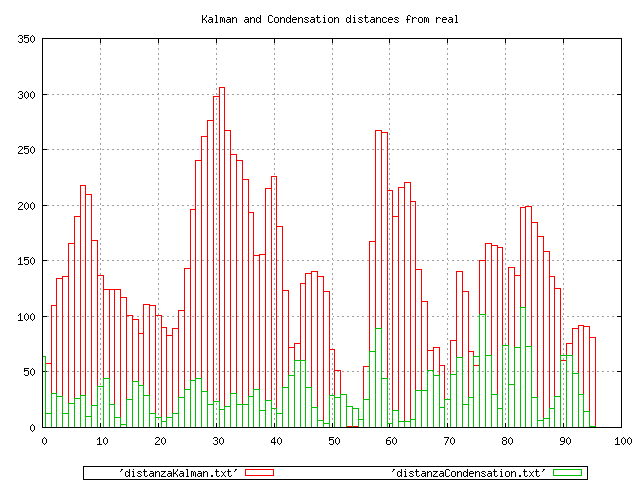
\includegraphics[scale=0.4]{../../esperimenti/tappeto_nozoom/mod_5-Q_1000-S_1000/plot-distances.png}
\caption{\textit{Test 7: Previsioni}}
\end{figure}

Statistiche:
\begin{itemize}
\item \begin{math} \bar \delta_K: 137 \end{math}
\item \begin{math} \bar \delta_C: 31\end{math}
\item \begin{math}(\sigma_x,\sigma_y)\end{math}: (56,40)
\end{itemize} 

Come prevedibile la rapidità di moto di questo oggetto mal si concilia una misurazione effettuata ad intervalli ampi. Entrambi i filtri si comportano in modo non proprio ottimale, in particolare Kalman perde quasi immediatamente l'oggetto. 

\newpage
\subsubsection{Test 8: MOD=2, Q=1000, S=1000}

\begin{figure}[hb]
\centering
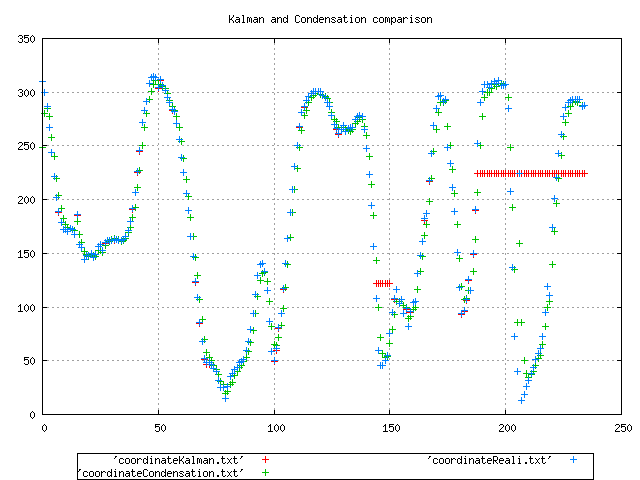
\includegraphics[scale=0.4]{../../esperimenti/tappeto_nozoom/mod_2-Q_1000-S_1000/plot.png}
\caption{\textit{Test 8: Tracciamento}}
\end{figure}

\begin{figure}[hb]
\centering
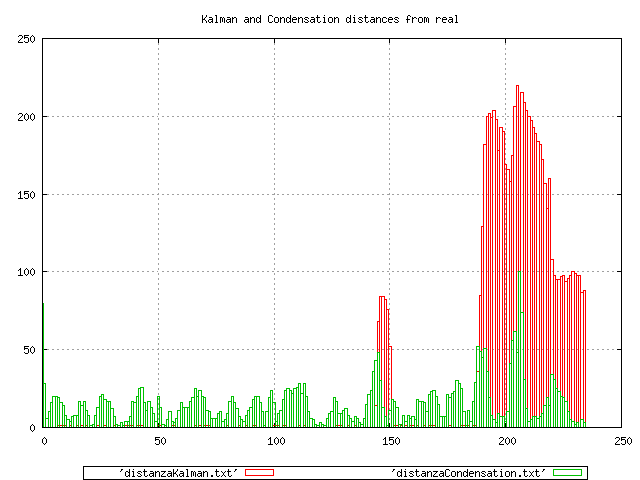
\includegraphics[scale=0.4]{../../esperimenti/tappeto_nozoom/mod_2-Q_1000-S_1000/plot-distances.png}
\caption{\textit{Test 8: Previsioni}}
\end{figure}

Statistiche:
\begin{itemize}
\item \begin{math} \bar \delta_K: 32 \end{math}
\item \begin{math} \bar \delta_C: 15 \end{math}
\item \begin{math}(\sigma_x,\sigma_y)\end{math}: (55,41)
\end{itemize}

La situazione decisamente migliora se invece campioniamo ogni 2 frames. Kalman fintato che non perde l'oggetto si comporta meglio del Condensation, in media però il Condensation risulta migliore.


\newpage
\subsubsection{Test 9: MOD=1, Q=2000, S=1000}

\begin{figure}[hb]
\centering
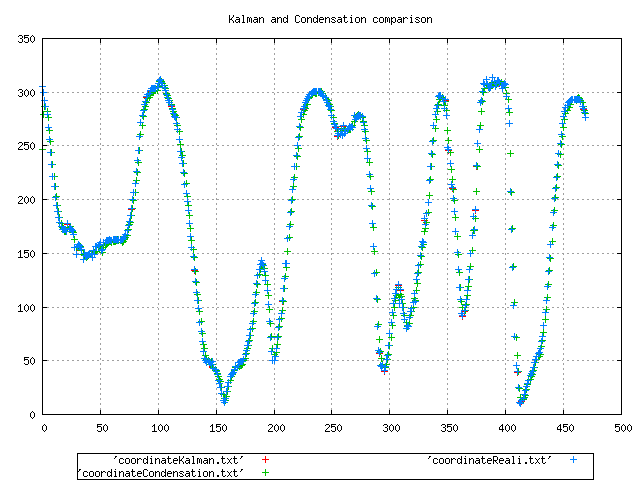
\includegraphics[scale=0.4]{../../esperimenti/tappeto_nozoom/mod_1-Q_2000-S_1000/plot.png}
\caption{\textit{Test 9: Tracciamento}}
\end{figure}

\begin{figure}[hb]
\centering
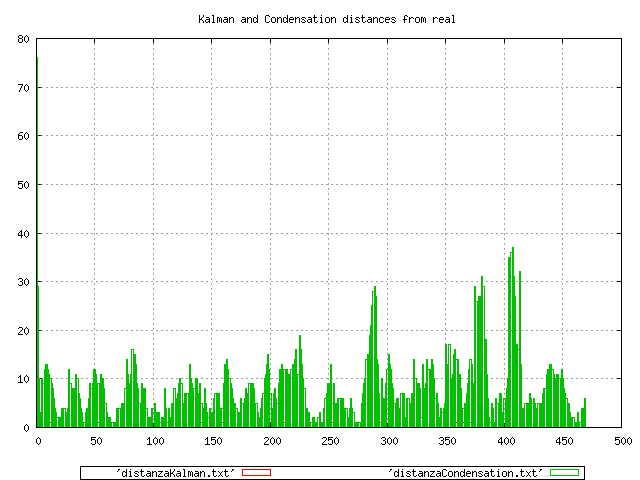
\includegraphics[scale=0.4]{../../esperimenti/tappeto_nozoom/mod_1-Q_2000-S_1000/plot-distances.png}
\caption{\textit{Test 9: Previsioni}}
\end{figure}

Statistiche:
\begin{itemize}
\item \begin{math} \bar \delta_K: 0 \end{math}
\item \begin{math} \bar \delta_C: 8 \end{math}
\item \begin{math}(\sigma_x,\sigma_y)\end{math}: (55,41)
\end{itemize}

Ingrandendo l'area di tolleranza per Kalman e prendendo la misura ogni frame Kalman traccia perfettamente il moto dell'oggetto e anche il Condensation migliora il proprio comportamento. Questa è una situazione ottimale, però decisamente poco realistica. Sono risultati che possiamo ottenere solo perchè stiamo tracciando il moto di un oggetto del quale conosciamo tutto dettagliatamente (Video Stream).

\newpage
\subsubsection{Test 10: MOD=1, Q=500, S=1000}

\begin{figure}[hb]
\centering
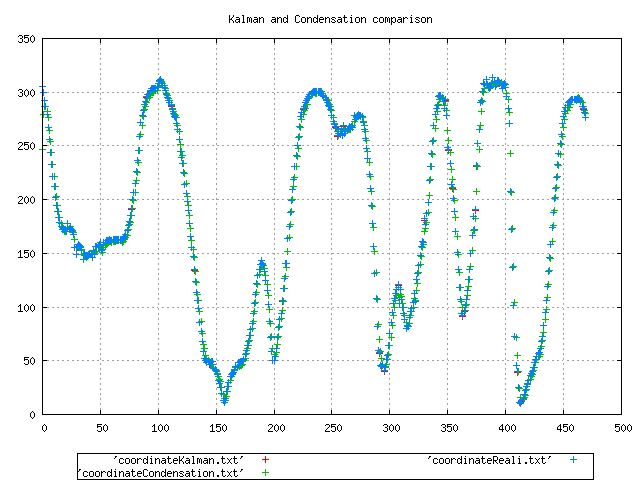
\includegraphics[scale=0.4]{../../esperimenti/tappeto_nozoom/mod_1-Q_500-S_1000/plot.png}
\caption{\textit{Test 10: Tracciamento}}
\end{figure}

\begin{figure}[hb]
\centering
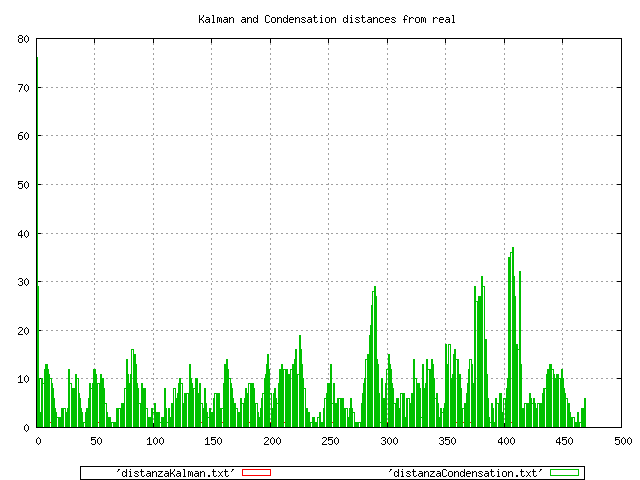
\includegraphics[scale=0.4]{../../esperimenti/tappeto_nozoom/mod_1-Q_500-S_1000/plot-distances.png}
\caption{\textit{Test 10: Previsioni}}
\end{figure}

Statistiche:
\begin{itemize}
\item \begin{math} \bar \delta_K: 0 \end{math}
\item \begin{math} \bar \delta_C: 8 \end{math}
\item \begin{math}(\sigma_x,\sigma_y)\end{math}: (55,41)
\end{itemize}

Campionando ogni frame, anche diminuendo l'area dell'ellisse di tolleranza per Kalman i risultati non cambiano.

\newpage
\subsection{Video: singlecar.avi}

\begin{itemize}
\item risoluzione: 648x484
\item fps: 30.00
\item durata: 33 s
\end{itemize}

Anche in questo caso il video è di un'automobilina radiocomadata ripresa dall'alto trasversalmente. A differenza che negli altri video non ci sono oggetti occludenti e il moto è piuttosto uniforme. L'automobilina, però, entra ed esce dalla scena più di una volta.

\begin{figure}[hb]
\centering
	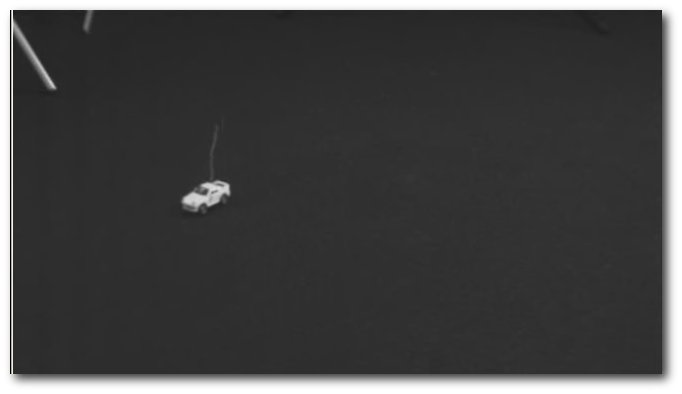
\includegraphics[scale=0.5]{singlecar.jpg}
\caption{\textit{movie12 screenshot}}
\end{figure}

\newpage
\subsubsection{Test 11: MOD=3, Q=1000, S=1000}

\begin{figure}[hb]
\centering
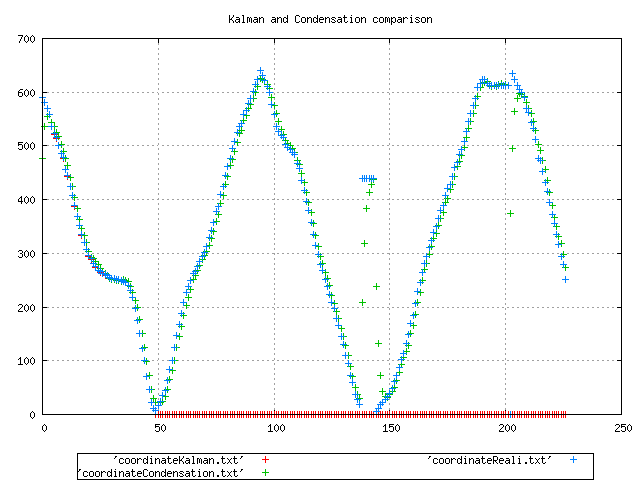
\includegraphics[scale=0.4]{../../esperimenti/single_car/mod_3-Q_1000-S_1000/plot.png}
\caption{\textit{Test 11: Tracciamento}}
\end{figure}

\begin{figure}[hb]
\centering
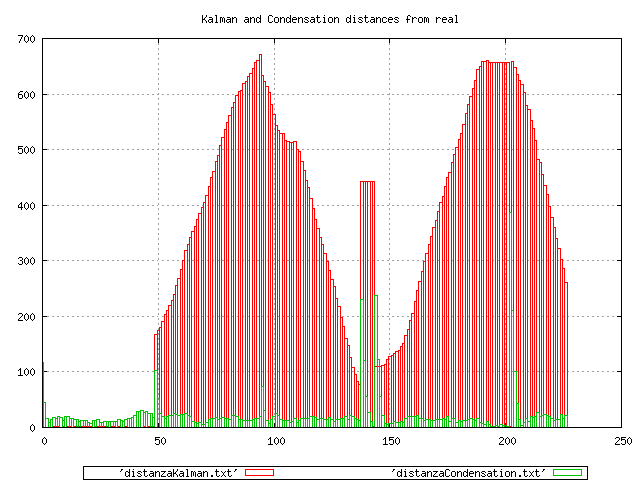
\includegraphics[scale=0.4]{../../esperimenti/single_car/mod_3-Q_1000-S_1000/plot-distances.png}
\caption{\textit{Test 11: Previsioni}}
\end{figure}

Statistiche:
\begin{itemize}
\item \begin{math} \bar \delta_K: 323  \end{math}
\item \begin{math} \bar \delta_C: 23 \end{math}
\item \begin{math}(\sigma_x,\sigma_y)\end{math}: (111,83)
\end{itemize}

In questo test si hanno i risultati più comuni: se l'oggetto scompare dalle scena e riappare in punti molto distanti da dove è scomparso il filtro di Kalman lo perde, ma quando l'oggetto è individuato correttamente Kalman è migliore del Condensation. 
Tuttavia in media il Condensation è molto più preciso nella predizione.

\newpage
\subsubsection{Test 12: MOD=10, Q=5000, S=1000}

\begin{figure}[hb]
\centering
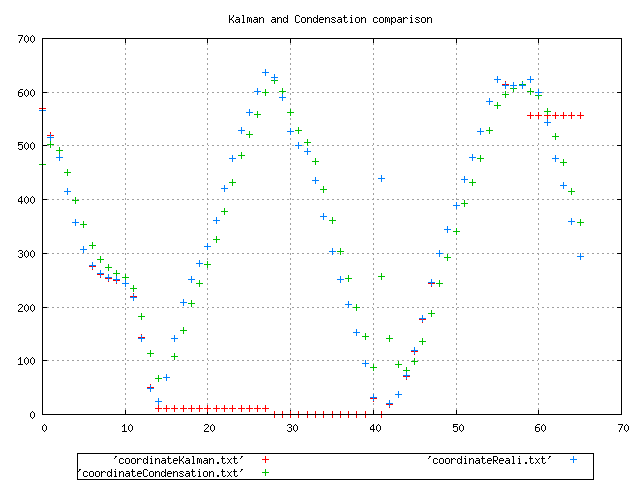
\includegraphics[scale=0.4]{../../esperimenti/single_car/mod_10-Q_5000-S_1000/plot.png}
\caption{\textit{Test 12: Tracciamento}}
\end{figure}

\begin{figure}[hb]
\centering
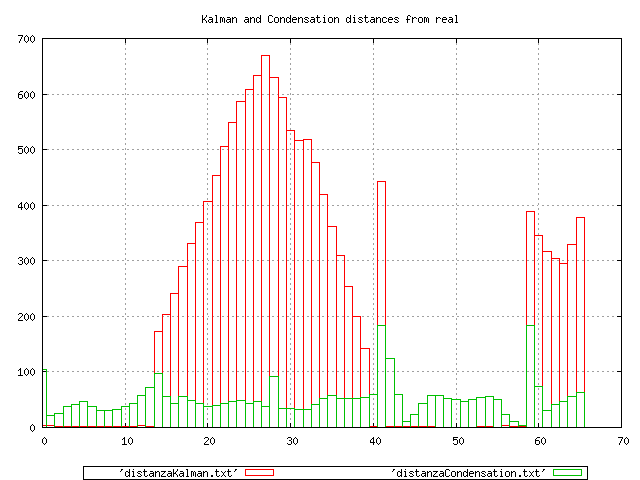
\includegraphics[scale=0.4]{../../esperimenti/single_car/mod_10-Q_5000-S_1000/plot-distances.png}
\caption{\textit{Test 12: Previsioni}}
\end{figure}

Statistiche:
\begin{itemize}
\item \begin{math} \bar \delta_K:  209 \end{math}
\item \begin{math} \bar \delta_C:  52 \end{math}
\item \begin{math}(\sigma_x,\sigma_y)\end{math}: (114,83)
\end{itemize}

Il video in questione si presta ad un tracciamento effettuato ad intervalli anche ampi poichè non ci sono brusche accelerazioni o frenate. Il problema principale sul filtro di Kalman resta che perde l'oggetto se scompare ed è perciò evidente la necessità di incrementare l'area di tolleranza per migliorare le prestazioni del filtro. 

\newpage
\subsubsection{Test 13: MOD=6, Q=1000, S=1000}

\begin{figure}[hb]
\centering
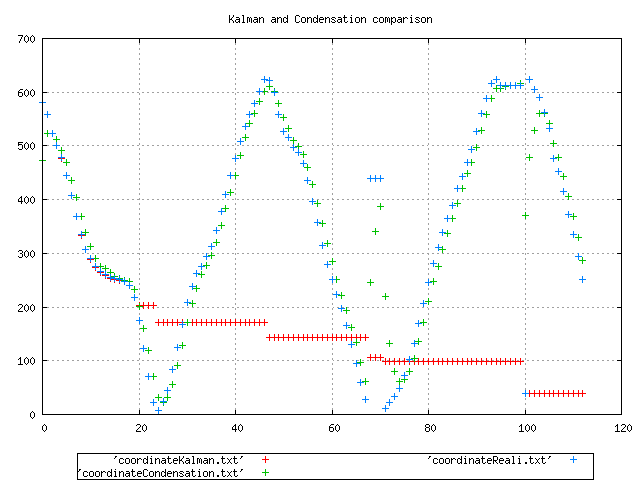
\includegraphics[scale=0.4]{../../esperimenti/single_car/mod_6-Q_1000-S_1000/plot.png}
\caption{\textit{Test 13: Tracciamento}}
\end{figure}

\begin{figure}[hb]
\centering
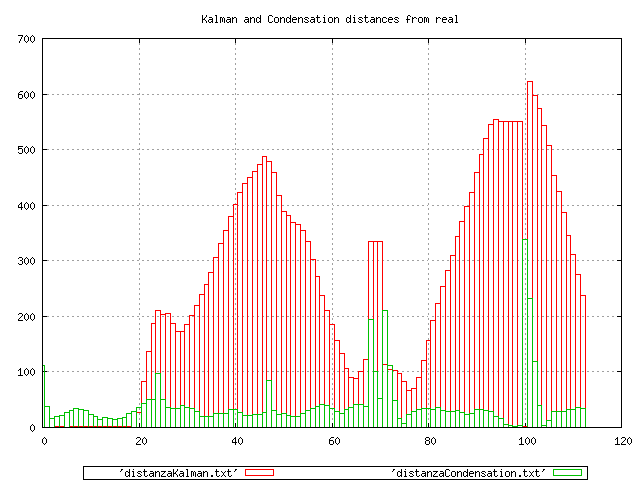
\includegraphics[scale=0.4]{../../esperimenti/single_car/mod_6-Q_1000-S_1000/plot-distances.png}
\caption{\textit{Test 13: Previsioni}}
\end{figure}

Statistiche:
\begin{itemize}
\item \begin{math} \bar \delta_K: 252 \end{math}
\item \begin{math} \bar \delta_C: 40 \end{math}
\item \begin{math}(\sigma_x,\sigma_y)\end{math}: (113,82)
\end{itemize}

Anche riducendo in numero di frames di campionamento la situazione non cambia molto, anzi per un caso crediamo dovuto alla natura del video stesso la situazione addirittura peggiora per il filtro di Kalman.
Decidiamo perciò di togliere il controllo sulla correttezza del rilevamento da parte di Kalman e ci poniamo come unico obiettivo quello di farlo lavorare in condizioni di minima tolleranza sull'errore.

\newpage
\subsubsection{Test 14: MOD=6, Q=1, S=1000}

\begin{figure}[hb]
\centering
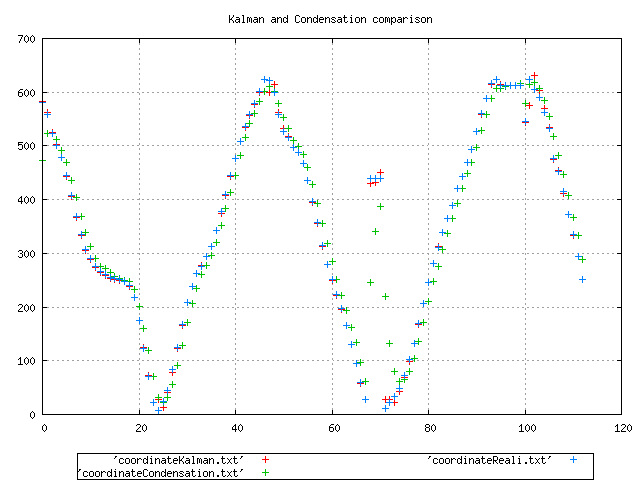
\includegraphics[scale=0.4]{../../esperimenti/single_car/mod_6-Q_1-S_1000/plot.png}
\caption{\textit{Test 14: Tracciamento}}
\end{figure}

\begin{figure}[hb]
\centering
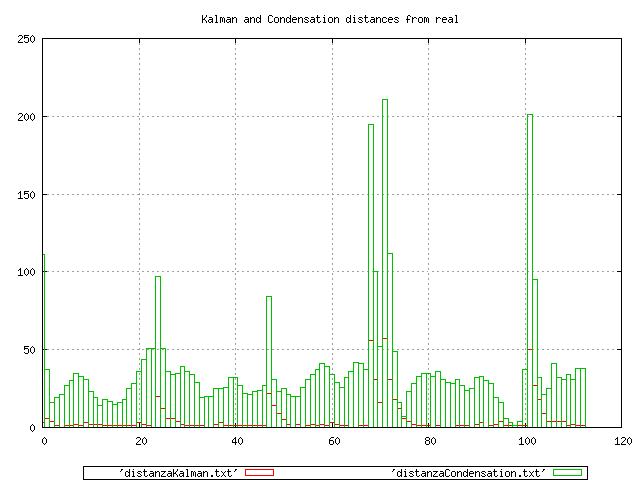
\includegraphics[scale=0.4]{../../esperimenti/single_car/mod_6-Q_1-S_1000/plot-distances.png}
\caption{\textit{Test 14: Previsioni}}
\end{figure}

Statistiche:
\begin{itemize}
\item \begin{math} \bar \delta_K: 5 \end{math}
\item \begin{math} \bar \delta_C: 37 \end{math}
\item \begin{math}(\sigma_x,\sigma_y)\end{math}: (113,82)
\end{itemize}

Togliendo il controllo sulla correttezza della predizione da parte di Kalman, se l'oggetto scompare siamo comuque in grado di tracciarlo (il filtro di Kalman lo ``insegue''). In media Kalman sbaglia pochissimo, il tracciamento è quasi perfetto.
L'obiettivo è ora quello di metterci in una situazione ipotetica in cui Kalman si comporta peggio del Condensation.

\newpage
\subsubsection{Test 15: MOD=6, Q=0.1, S=1000}

\begin{figure}[hb]
\centering
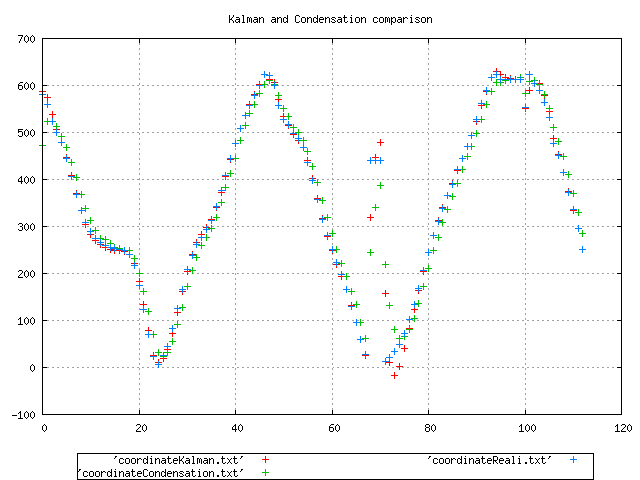
\includegraphics[scale=0.4]{../../esperimenti/single_car/mod_6-Q_0.1-S_1000/plot.png}
\caption{\textit{Test 15: Tracciamento}}
\end{figure}

\begin{figure}[hb]
\centering
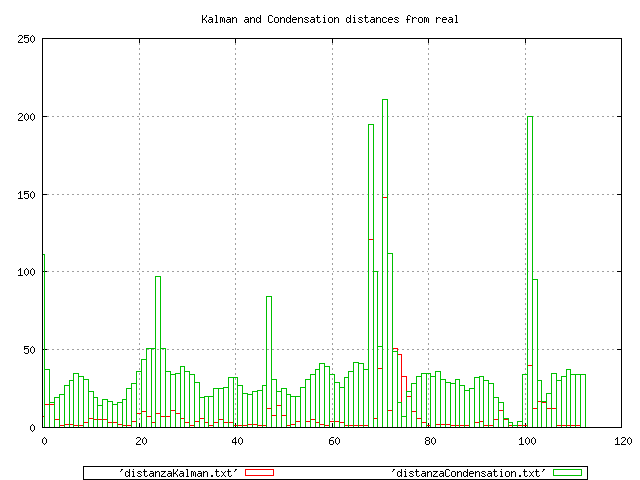
\includegraphics[scale=0.4]{../../esperimenti/single_car/mod_6-Q_0.1-S_1000/plot-distances.png}
\caption{\textit{Test 15: Previsioni}}
\end{figure}

Statistiche:
\begin{itemize}
\item \begin{math} \bar \delta_K: 8 \end{math}
\item \begin{math} \bar \delta_C: 37 \end{math}
\item \begin{math}(\sigma_x,\sigma_y)\end{math}: (113,82)
\end{itemize}

Riduciamo l'errore consentito sulla predizione, l'ellisse di tolleranza si riduce imponendo a Kalma di sbagliare il meno possibile. In questo test i risultati ottenuti non si discostano molto da quelli precedenti, l'oggetto è sempre tracciato ottimamente dal filtro di Kalman.

\newpage
\subsubsection{Test 16: MOD=6, Q=0.001, S=1000}

\begin{figure}[hb]
\centering
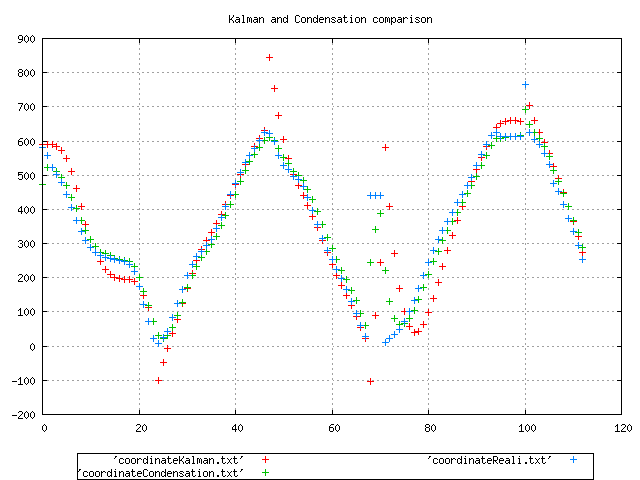
\includegraphics[scale=0.4]{../../esperimenti/single_car/mod_6-Q_0.001-S_1000/plot.png}
\caption{\textit{Test 16: Tracciamento}}
\end{figure}

\begin{figure}[hb]
\centering
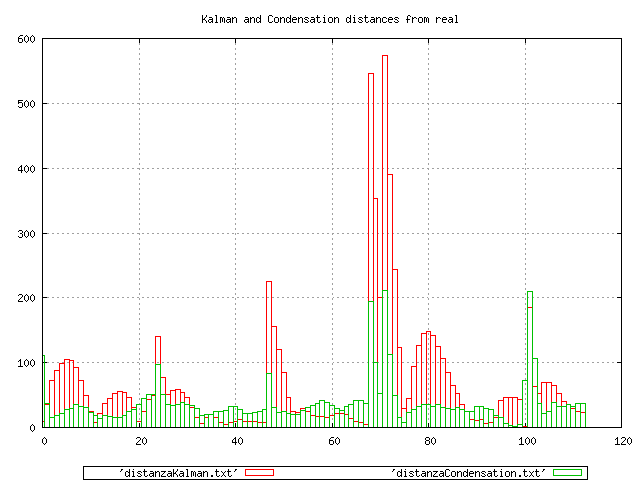
\includegraphics[scale=0.4]{../../esperimenti/single_car/mod_6-Q_0.001-S_1000/plot-distances.png}
\caption{\textit{Test 16: Previsioni}}
\end{figure}

Statistiche:
\begin{itemize}
\item \begin{math} \bar \delta_K: 66 \end{math}
\item \begin{math} \bar \delta_C: 43 \end{math}
\item \begin{math}(\sigma_x,\sigma_y)\end{math}: (114,82)
\end{itemize}

Come previsto il filtro di Kalman comincia finalmente a peggiorare il proprio comportamento anche se in media è sempre migliore dell'altro. 

\newpage
\subsubsection{Test 17: MOD=6, Q=0.0001, S=1000}

\begin{figure}[hb]
\centering
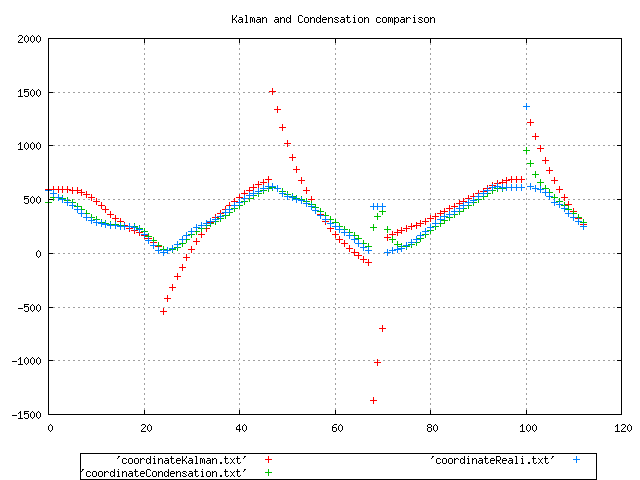
\includegraphics[scale=0.4]{../../esperimenti/single_car/mod_6-Q_0.0001-S_1000/plot.png}
\caption{\textit{Test 17: Tracciamento}}
\end{figure}

\begin{figure}[hb]
\centering
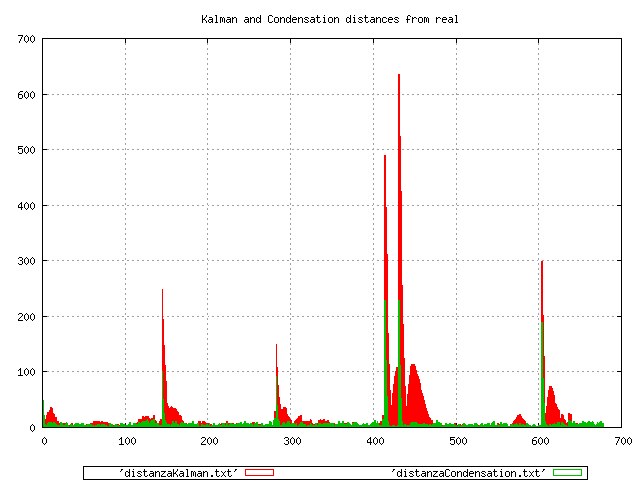
\includegraphics[scale=0.4]{../../esperimenti/single_car/mod_1-Q_0.0001-S_1000/plot-distances.png}
\caption{\textit{Test 17: Previsioni}}
\end{figure}

Statistiche:
\begin{itemize}
\item \begin{math} \bar \delta_K: 179 \end{math}
\item \begin{math} \bar \delta_C: 43 \end{math}
\item \begin{math}(\sigma_x,\sigma_y)\end{math}: (114,83)
\end{itemize}

In questo test Kalman non riesce più a tracciare correttamente l'oggetto. Appare qui evidente come alcune zone si dimostrino particolarmente critiche per il filtro di Kalman.

\newpage
\subsubsection{Test 18: MOD=1, Q=0.0001, S=1000}

\begin{figure}[hb]
\centering
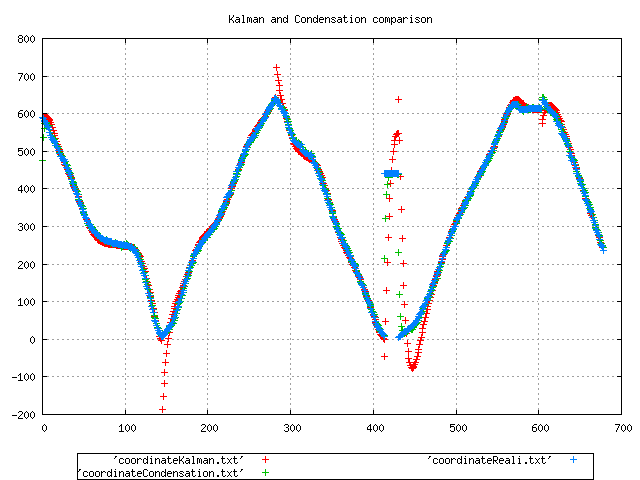
\includegraphics[scale=0.4]{../../esperimenti/single_car/mod_1-Q_0.0001-S_1000/plot.png}
\caption{\textit{Test 18: Tracciamento}}
\end{figure}

\begin{figure}[hb]
\centering
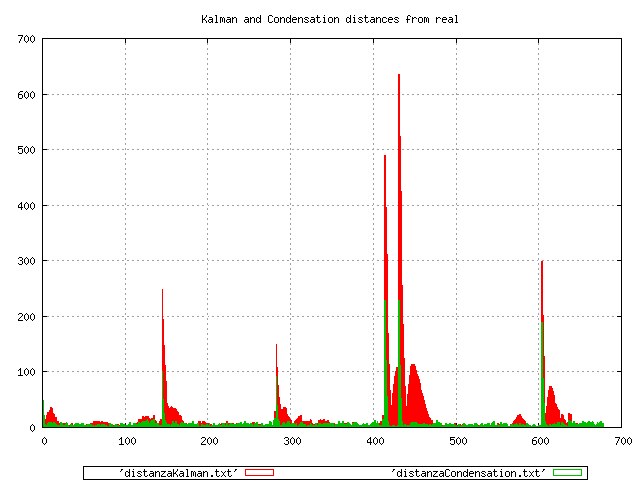
\includegraphics[scale=0.4]{../../esperimenti/single_car/mod_1-Q_0.0001-S_1000/plot-distances.png}
\caption{\textit{Test 18: Previsioni}}
\end{figure}

Abbiamo variato anche la frequenza di campionamento.
Qui il comportamento di Kalman è migliore rispetto al test precedente ed è più chiaro come Kalman si trovi in difficoltà soprattutto nel tracciare zone di non linearità del moto dell'oggetto. (smoothness)

Statistiche:
\begin{itemize}
\item \begin{math} \bar \delta_K: 22 \end{math}
\item \begin{math} \bar \delta_C: 8\end{math}
\item \begin{math}(\sigma_x,\sigma_y)\end{math}: (111,85)
\end{itemize}


     %%%%%%%%%%%%%%%%%%%%
     %                  %
     %  capitolo1.tex   %
     %                  %
     %%%%%%%%%%%%%%%%%%%%

\section{Sviluppo dell'applicativo}

\subsection{Obiettivi}
L' obiettivo del software è quello di realizzare un applicativo che esegua \textit{model based tracking} \ref{modelTracking} sulla base di un video passatogli come ingresso. Più nel dettaglio l'applicazione esegue il tracciamento tramite il filtro di Kalman \cite{kalman-intro} e il ConDensaTion \cite{kalman-condense}, in maniera tale da poter confrontare le prestazioni dell' uno e dell'altro.\\
Altri requisiti funzionali sono quelli di:

\begin{itemize}
 \item  fare scegliere all'utente l'oggetto da tracciare in caso di tracking multiplo: in questo caso il software si ferma sul primo frame del video, dando possibilità di scegliere l'oggetto di cui si vuol fare il tracciamento. Per migliorare la selezione di un oggetto, vengono evidenziati dei un puntini gialli in corrispondenza del blob identificato. Vedi figura \ref{fig:scelta2blob}

\item tracciare a video l'andamento dei due algoritmi, evidenziandoli con colori differenti; visualizzare un' ellissi per ogni algoritmo che indichi la varianza del vettore di stato per quel tipo di tracking.

\item fornire un output razionalizzato su terminale e su filesystem per verificare rispettivamente la corretta esecuzione degli algoritmi e per avere un riscontro finale sulle performance e l'accuratezza di ognuno. Successivamente parsare i suddetti file per una rappresentazione grafica dell'accuratezza dei due metodi di tracking.

\item progettare e realizzare l'applicazione in maniera tale che possa essere compilata ed eseguite su piattaforme diverse.


\end{itemize}

I dettagli implementativi di questi punti sono rimandati alla sottosezione  \ref{ControlFlow}

\begin{figure}[hb]
\centering
	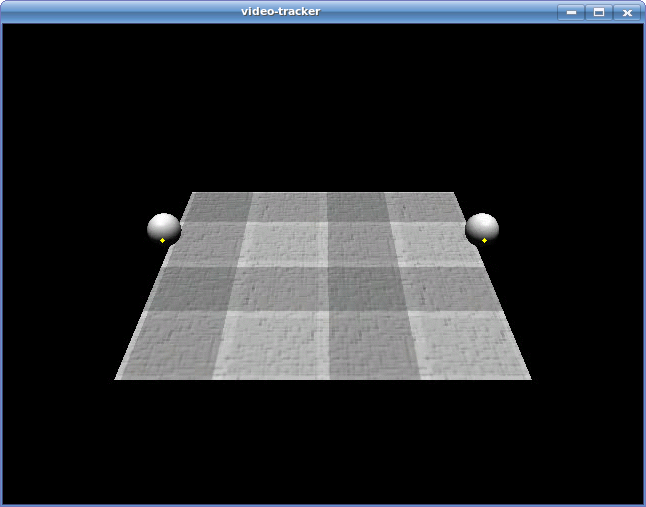
\includegraphics[scale=0.5]{doppiascelta.png}
\caption[Esempio di scelta tra due blob]{\textit{Esempio di scelta tra due blob su tracking multiplo: l'utente ha la possibilità di sccegliere su quale blob effettuare il tracciamento semplicemente cliccando vicino ad uno dei punti gialli. Il Sistema automaticamente selezionerà il blob più vicino attraverso il calcolo della distanza euclidea}\label{fig:scelta2blob}}
\end{figure}


\'E bene sottolineare che il video in ingresso possiede delle restrizioni: infatti affinchè il \textit{background subtraction} lavori in maniera ottima, è necessario che il video:
\begin{itemize}
 \item possieda semper uno sfondo fisso o che comunque non vari durante la ripresa. Cambiare sfondo sarrebbe come rinizializzare l'agoritmo per il detecting dei blob.
\item possieda un numero ( $n > 40 $ ) di frame inziale che mostrino solo il background per facilitare il calcolo della \textit{ground truth}, cioè del blob osservato da cui prendere le misure per i due algoritmi.
\item sia stato registrato da una postazione fissa e quindi che la telecamera di ripersa non introduca nel video un moto relativo.
 \end{itemize}

Qualsiasi video che rispetta questi tre vincoli è considerato non solo adeguato, ma ottimale per effettuare il tracking con la nostra applicazione.




%ingresso video fatto in un certo modo (sfondo fisso, tot frame di background iniziale, telecamera fissa)

%uno o + oggetti in moto

%permette di selezionare QUALE oggetto seguire, farne il tracciamento reale, ottenere le predizioni secondo k e c, e raccoglierne dati e risultati per la realizzazione di grafici

%intro utilizzo librerie utilizzate intel openCV
\subsection{Librerie Intel OpenCV}
Per svilluppare l'applicazione sono state utilizzate le libreria \textit{OpenCV}, emergente nel campo della \textit{computer vision}  e sviluppata da Intel sotto una licenza di tipo OpenSource, compatibile con la GNU GPL.
\'E bene però prima fare chiarezza sull'uso e lo scopo di queste librerie.\\
La capacità di interpretare ed utilizzare correttamente le informazioni acquisite da una videocamera o fotocamera attualmente presenta molti problemi insoluti. Convertire un’immagine in informazioni “oggettive” astraendone il contenuto dalla pura rappresentazione luminosa, sebbene sia un’operazione banale per un cervello umano adulto è, a tutt’oggi, un problema di elevata complessità per un sistema automatico.
Oltretutto il campo di ricerca è evidentemente molto giovane, con meno di trent’anni di esperienza. In quest’ottica si inserisce la necessità di una base comune di potenti strumenti analitici, primo dei quali una \textbf{libreria} che raccolga le funzionalità degli algoritmi più utilizzati e citati in letteratura, oltre che una serie di formati di rappresentazione dei dati secondo standard aperti e condivisi.\\
Le librerie OpenCV (Open Source Computer Vision) nascono appunto a questo scopo; lo sviluppo prende le mossa da un gruppo di ricerca sponsorizzato da Intel. E’ infatti parzialmente basata sulla \textit{Intel Image Processing Library (IPL)}: tale prodotto è oggi integrato nella libreria commerciale IIPP (Intel Integrated Performance Primitives), con cui conserva piena compatibilità e che può eventualmente rendere disponibili un completo ventaglio di funzioni più specifiche.\\
Tra i punti di forza sottolineiamo inoltre la politica di licenza utilizzata, in stile BSD e definita nella ``Intel License Agreement For Open Source Computer Vision Library'', completamente compatibile con la licenza GPL. A grandi linee questo permette una libera ridistribuzione sia in forma sorgente che binaria, anche all’interno di prodotti commerciali, a condizione di mantenere le note di copyright e di non utilizzare il nome Intel a scopo promozionale di prodotti derivati.\\
Inoltre un' altra potenzialità offerta è la caratteristica di essere \textit{cross-platform}: cioè possono essere compilate e usate sia sotto sistema operativo Microsft Windows che GNU/Linux. Questa caratteristica le rende molto appetibili per i requisiti di portabilià che ci eravamo prefissi di raggiungere.\\ Da notare che le librerie sono scritte in linguaggio C e non fanno uso quindi di un linguaggio orientato agli oggetti.

\subsubsection{Aree funzionali delle librerie}
Si vuol chiarire subito un fatto che può essere causa di equivoci: con il termine ``libreria grafica'' infatti si identificano genericamente almeno tre famiglie di librerie, i cui scopi sono sostanzialmente differenti:
\begin{enumerate}
 \item  I Toolkit, ovvero librerie di primitive per la creazione di oggetti grafici di interfaccia (finestre, icone, bottoni,ecc). Parzialemente ricoperto in OpenCV dalle HighGui.
\item Librerie di rendering e multimedia, come DirectX e OpenGL, orientate alla massima performance nella creazione di effetti poligonali o vettoriali. L’utilizzo più comune è teso all’ottenimento di elevate prestazioni    grafiche sfruttate ad esempio nei videogiochi o nelle applicazioni multimediali.
\item  Librerie di gestione hardware grafico, come digitalizzatori e frame-grabber. Pur includendo tipicamente una base di funzioni di trattamento sono generalmente da considerarsi come API dei relativi driver hardware.
\end{enumerate}

Le OpenCV, pur includendo alcune funzionalità tipiche di ciascuna delle famiglie citate \footnote{vedi esempio delle HighGui}, non fanno parte di nessuno di questi gruppi. L’utilizzo primario è infatti quello collegato alla visione artificiale, il cui problema principale, come già visto, è quello di estrarre da immagini/video dati significativi, trattabili in modo automatico. Tale campo di studio trova le sue applicazioni più comuni nella robotica, nei sistemi di  videosorveglianza evoluti e nei sistemi di monitoraggio e sicurezza, oltre che in ogni sistema di archiviazione automatica di informazioni visive.\\
La libreria include attualmente più di 300 funzioni, che coprono le più svariate esigenze di trattamento di immagini, comprese funzioni matematiche ottimizzate (elevamento a potenza, logaritmi, conversioni cartesiane-polari, ecc.) ed  un completo pacchetto di algebra matriciale, sviluppato funzionalmente al resto del sistema.\\

La principale categoria di uso rimane comunque il processing di tipo real-time su immagini e video. \\
Una panoramica generale delle librerie comprende questi aspetti della computer vision:
\begin{enumerate}
\item Human-Computer Interface (HCI)
\item Object Identification
\item Segmentation and Recognition
\item Face Recognition e Gesture Recognition
\item Motion Tracking  riferimento al nostro progetto
\end{enumerate}

%descrivere un po queste aree e dove si usano noi nel nostro progetto.




\subsubsection{Riferimenti}

Come molti progetti opensource in maturazione \footnote{La versione 1.0 ufficiale è stata rilasciata nel tardo 2006; parte del progetto è stato scritto con librerie in beta testing} è stata carente la parte che riguarda la documentazione. Nonostante la presenza di un colosso alla spalle e di una struttura basata sul modello wiki, la documentazione ufficiale in pdf e html, anche se facilmente fruibile, non è stata sufficiente per colmare le lacune iniziali. Per questo motivo è stato effettuato un grosso lavoro di studio per capire il funzionamento del toolkit OpenCv, che spesso è terminato con la ricerca di documentazione in website asiatici, dove sembra che queste librerie siano molto gradite.\\
Alcuni riferimenti importanti per OpenCV:
\begin{itemize}
 \item \htmladdnormallink{Sito web ufficiale}{http://www.intel.com/technology/computing/opencv/index.htm}
\item \htmladdnormallink{Portale di wiki}{http://opencvlibrary.sourceforge.net}
\item \htmladdnormallink{ OpenCv - Groups Community}{http://tech.groups.yahoo.com/group/OpenCV/}
\end{itemize}

 
\subsection{Control Flow del programma}\label{ControlFlow}
%intro del ciclozzo FOR e che cosa viene fatto in ordine con l'acquisizione frame/frame del video
Come citato precedentemente, si va ora a evidenziare quelli che sono stato gli accorgimenti tecnici per implementare il nostro software di comparazione tra Kalman e Condensation.\\
Si cercherà di non riportare tutto il codice sorgente, ma di evidenziare solo spezzoni di esso, che possono fornire preziose informazioni sulla struttura. \'E bene sottolineare che in linea con le OpenCV, la parte principale del software non è stata sviluppata secondo il paradigma Object Oriented, ma si è usato la razionalizzazione delle strutture dati in classi solo quando necessario.
Il nucleo centrale dell' applicazione è il \textbf{ciclo for} che dipende dalla lunghezza del video da analizzare. Ogni calcolo verrà fatto quindi in \textbf{modalità online}, cioè ad ogni passo dentro il ciclo stesso. Ne listato di pseudo codice sottostante è riprotato l'idea dell' andamento dell'applicativo. 
\newpage

\lstset{language=c++}
\lstset{commentstyle=\emph}
\begin{lstlisting}[frame=l,caption=Nucleo dell'Applicazione - execute.cpp ,breaklines=true,basicstyle=\small]{Nucleo dell'Applicazione - execute.cpp}

void execute( file ){

	video = captureFromAvi( file )
	
	initBackgroundSubtraction( video )

	for( int fr = 1; frame = captureNextFrame( video ), fr++ ){
	
		updateBackgroundSubtraction( frame )
		
		if ( frame == FIRST_FRAME){
			
			blobs = getBlobSelectedFromUser( frame )
	
			initKalman( blobs );
			
			initCondensation( blobs );
		}
	
		updateKalman();
		updateCondensation();
	}
}

\end{lstlisting}

\subsubsection{Back subtraction}
%realizzazione online del backsub, librerie eccetera
\subsubsection{Predizione}
\subsubsection{Rappresentazione della predizione}
\subsubsection{HiGui}
\subsubsection{Scripting GNUPlot}


% \chapter{Il software libero nel sistema giuridico informatico}

Appurate le definizioni di forma di tutela della Proprietà Intellettuale come copyright, brevetto e marchio nel capitolo 1 e la storia dei brevetti applicati software nei mercati più sviluppati come USA e UE nel capitolo 2, si sfrutta i seguenti due capitolo dell'elaborato per approfondire il dibattito sulla tutela del software che oscilla tra copyrigt e brevetti.

In particolare nel capitlo 3 si approfondirà come il movimento opensource stia cercando di difendersi dalla brevettazione del software attraverso la licenza madre copyleft \textit{par excellence}: la GPL, modificata di recente per questo motivo approdando alla terza versione.
In questo trattato non si approfondiranno nè i concetti di opensource o free software nè il concetto di copyleft, che invece possono essere conosciuti rispettivamente attraverso la lettura di \cite[Compendio di libertà informatica e cultura open]{Aliprandi-compendio} e \cite[Copyleft e Opencontent]{Aliprandi-copyleft}

Il capitolo 4 invece sarà più pratico: si metteranno in luce delle conseguenze che la brevettazione software apporta sia nel software libero che in quello proprietario e commerciale; quindi si farà un esempio di brevetto, verrà spiegato e si vedrà le conseguenze portati in USA e in UE.

Adesso si va ad approfondire alla luce di quanto visto fino ad ora, come si tutela il \textit{free software} nel sistema giuridico informatico.


\section{Le licenze libere}
Breve introduzione
	\subsection{La licenza GPL}
	breve
\section{L'approccio ai brevetti della nuova licenza GPLv3}
va letta la GPL3 e spulciata per quanto riguarda i brevetti riportando magari qualche tratto saliente.
\section{Un esempio di brevetto vincolato dalla GPLv3}
idem


%\chapter{Un esempio concreto: il caso MP3}
Per rendere chiara e comprensibile la trattazione sarà portata come esemplificativa uno delle questioni più famose e rilevanti nella storia della brevettazione software, sia per l'importanza dell'invenzione sotto brevetto, sia per la rilevanza economica che ha avuto la causa giudiziaria di violazione di brevetto che ha colpito una delle più importanti aziende informatiche: Microsoft Corporation.

Rilevante sarà anche l'analisi del comportamento che deve essere tenuto nelle varie regioni mondiali in virtù della valenza o meno del suddetto brevetto: per chiarire questa problematica sarà portato come esemplare il comportamento della distribuzione GNU/Linux più diffusa al momento, Ubuntu Linux\cite{ubuntu}.

\section{Cos'è l'algoritmo di compressione MP3}
La discussione di questo capitolo verte su uno degli algoritmi più importanti della storia informatica degli ultimi tempi: l'algoritmo di compressione audio \textit{MPEG-1/2 Audio Layer 3}, comunemente noto come MP3. Questo algoritmo di compressione è diventato noto per la sua capacità di ridurre drasticamente la quantità di dati richiesti per la riproduzione di un suono, mantenendo comunque una riproduzione fedele del suono originario. Nei moderni codificatori MP3 gli algoritmi più efficaci fanno di tutto per assicurare che i suoni rimossi siano quelli che non possono essere rilevati dall'orecchio umano. Questo risultato è stato ottenuto anche grazie alla scienza della psicoacustica.

Nonostante ne siano stati riconosciuti molti difetti, diversi dei quali superati anche da algoritmi successivi ed alternativi (si pensi all'algoritmo \textit{AAC MPEG-4} oppure all'\textit{Ogg Vorbis}) il formato .mp3 (classico dei files compressi con tale algoritmo) risulta ancora il più diffuso in campo musicale, e ciò spiega la portata economica che può comportare l'eventuale copertura brevettuale sull'invenzione.
\section{Il brevetto sull'MP3}\label{mp3-patent}
La Thomson Consumer Electronics è la proprietaria principale del brevetto di MPEG-1/2 Layer 3 in U.S.A. e Giappone, e ha raccolto in un apposito sito (\textit{http://www.mp3licensing.com/}) tutte i brevetti relativi all'MP3 che detiene (svariati validi anche in UE), e una riepilogativa tabella delle royalties che le aziende devono pagare per utilizzare codificatori e decodificatori di MP3.
\begin{figure}[hb]
	\begin{center}
		
\includegraphics[scale=0.75]{figure/mp3.jpg}
	\end{center}
	\caption{\textit{Il logo del sito Thomson sui brevetti MP3}}
\end{figure}
\subsection{Ricerca del brevetto}

\subsection{Termini del brevetto}

\subsection{Aree di valenza e royalties}

\section{Il delicato rapporto tra Microsoft ed il formato MP3}
Scendendo nelle notizie di attualità è comune trovare, in campo tecnico/ingegneristico, notizie di violazioni di brevetto, di violazione di proprietà intellettuali e simili. Un po' meno raro è trovare eventi che vedano implicati i brevetti software, specialmente in Europa, dove, come abbiamo visto, sono quasi impossibili da ottenere. 

\`E normale quindi che faccia scalpore quando un tribunale emette una sentenza di violazione di brevetto informatico contro una azienda; è ancora più normale che l'interesse salga a livelli inauditi se l'azienda coinvolta è la più fiorente in campo informatico, e viene condannata ad una pena pecuniaria pari al fatturato di una decina di anni di una azienda normale. Stiamo parlando della Microsoft, e della \textit{querelle} giudiziaria che l'ha vista protagonista con Alcatel-Lucent.

La questione è spinosa in quanto non vede solo motivazioni giuridiche tra i proprietari originari del brevetto ed il presunto violatore, ma vede di fronte al presunto violatore delle enormi aziende che hanno inglobato in percentuali diverse le originali proprietarie del brevetto, lasciando innescare quindi procedure economico/giudiziarie dalla portata enorme.

Nel caso di MP3, come è stato detto nella sezione \ref{mp3-patent}, il principale detentore della proprietà brevettuale è Thomson Consumer Electronics, ma non è affatto ne' l'unica ne' l'originaria proprietaria. Gli algoritmi di base di MP3 sono stati sviluppati originariamente in collaborazione tra il Fraunhofer Institute e gli ex-Bell Laboratories. Il primo gruppo a rilasciare un encoder fu il Fraunhofer Institute nel 1994, e Microsoft ha sempre sostenuto di aver ottenuto in licenza la tecnologia proprio da quest'ultimo, pagandola ben 16 milioni di dollari ed integrandola nei sistemi operativi Windows attraverso i codec e il lettore software Windows Media Player.

Thomson è di fatto la società che al momento controlla il Fraunhofer Institute, mentre Alcatel-Lucent al momento detiene la proprietà dei Bell Laboratories.

Proprio Alcatel-Lucent nel 2003 ha trascinato in tribunale i produttori di PC Dell e Gateway per l'utilizzo illegittimo dei suoi brevetti. Microsoft, in accordo con i patti di indennizzo stretti con le due società, ha offerto loro protezione legale ed ha ottenuto come contropartita la denuncia di Alcatel per la violazione degli accordi di sfruttamento dei brevetti sulla console Xbox 360. Le due aziende avevano stretto un'intesa sulla prima Xbox ma Alcatel-Lucent ha sostenuto davanti al giudice - e ha infine ottenuto una sentenza a proprio favore - che l'accordo non comprendeva la nuova versione; in tutto la disputa riguardava ben quindici violazioni di brevetto, e dopo il rigetto delle prime due accuse, nel Febbraio del 2007 è arrivata la notizia di una sconfitta giuridica per la Microsoft, per la violazione appunto del brevetto riguardante MP3. La sanzione prevedeva una multa per più di un miliardo e mezzo di dollari, valutati i benefici sfruttati abusivamente da Microsoft nel proprio sistema, valutata la diffusione del formato MP3 e la diffusione del sistema Microsoft stesso.

Il motivo principale della diatriba è strettamente legato alle royalties\footnote{Con il termine royalty si indica il pagamento di un compenso al titolare di un brevetto o una proprietà intellettuale, con lo scopo di poter sfruttare quel bene per fini commerciali.} che le aziende devono pagare per poter utilizzare il formato MP3. Come si può vedere nell'elenco pubblico disponibile nel sito Thomson già citato in precedenza, Microsoft risulta considerata tra le aziende autorizzate all'utilizzo della tecnologia; Alcatel, cercando di sfruttare altri processi già aperti contro la casa di Redmond ha tentato di avvalersi del presunto diritto di riscuotere ulteriori royalties sul formato, in virtù dell'acquisizione dei Bell Laboratories.

La questione, ancora non definitivamente sciolta in quanto è ancora possibile un ulteriore grado di giudizio, ha visto la sentenza in appello ribaltare, e di fatto annullare, la sentenza contro Microsoft, riconoscendo sufficiente il pagamento del brevetto presso uno dei proprietari legittimi.

Non ha comunque avuto vita facile la casa di Redmond verso questo formato di compressione audio. Mentre negli Stati Uniti, dove vige il brevetto, ha dovuto sostenere questo lungo processo (non ancora terminato), risulta interessante vedere anche il trattamento che le è stato riservato nell'Unione Europea, dove i brevetti principali dell'MP3 non sono validi.

La Microsoft, dovendo produrre un sistema operativo con bacino d'utenza mondiale, ha inizialmente provato a ``boicottare'' questo formato, cercando di far abituare i suoi utenti al suo formato proprietario (.wma) senza fornire il proprio sistema operativo del supporto per MP3. Questo la lasciava libera negli Stati Uniti dove il brevetto l'avrebbe obbligata al pagamento delle royalties, ma l'ha messa in cattiva luce verso l'antirtrust europeo. 

Il formato .wma a differenza dell'MP3 (che è a specifiche aperte), è a specifiche chiuse e quindi impone all'utente l'utilizzo del software pensato e realizzato dalla stessa Microsoft; d'altro canto la possibilità di essere il produttore del sistema operativo distribuito per più del 90\% sul pianeta aveva indotto la Microsoft a pensare di poter innestare il boicottaggio tramite la procedura di ``abitudine'' degli utenti. 

Sotto la presidenza di Mario Monti, l'antitrust europeo ha comminato alla Microsoft una multa per abuso di posizione dominante con il massimo della sanzione, il 10\% del fatturato. Microsoft è stata costretta ad abilitare l'installazione su Windows di lettori audio diversi dal nativo Windows Media Player, venduto insieme al sistema operativo ad inizialmente l'unico player disponibile sulla piattaforma (e come detto senza il supporto a MP3). Questi software invece dispongono della possibilità di ascoltare l'mp3 e altri formati diversi dal ``.wma'': alla fine, lo stesso software "Windows Media Player" è stato modificato per la lettura di molti codec e la loro masterizzazione, fra i quali c'è l'mp3.

La diatriba tra Microsoft ed il formato MP3 sembra adesso sistemata, in modo positivo per l'azienda negli Stati Uniti ed in modo negativo nell'Unione Europea; la Microsoft resta comunque una delle principali sostenitrici della brevettazione software, intesa come baluardo difensivo del software proprietario e come difesa estrema contro l'avanzata del software libero ed open source. 

Questa presa di posizione sembra quasi confermare la tesi espressa recentemente\footnote{Dal blog personale  http://www.markshuttleworth.com/archives/118} da Mark Shuttleworth, fondatore di Ubuntu, che sostiene quanto non sia la Microsoft stessa la più grossa nemica dello sviluppo open source, ma piuttosto lo sia la possibilità di poter brevettare software in alcuni paesi, che mette moltissime aziende e laboratori di piccole o medie dimensioni in virtù di chiedere royalties pesantissime agli sviluppatori; Microsoft al pari di molte altre aziende e società open source che producono tecnologia (ed anche di più, considerata la distribuzione di Windows), spende cifre sempre più salate per difendersi dalle cause legali relative ai brevetti e per il pagamento delle royalties: questo ha la possibilità di interferire con i piani di sviluppo e rilascio del software, danneggiandola economicamente e portandola con tutta probabilità alla difesa della non brevettabilità del software nel mondo.

Lo stesso Shuttleworth traccia con la propria distribuzione Linux la strada per poter ``convivere'' pacificamente con MP3, senza di fatto pagare royalties o piegarsi a logiche di brevetto.
\section{Il caso Ubuntu: come utilizzare gli MP3 senza violare il brevetto}
Ubuntu è una distribuzione GNU/Linux nata nel 2004 e basata su Debian, che si concentra sulla facilità di installazione e d'uso e sul rilascio regolare (semestrale) delle nuove versioni. 

Finanziata dalla società Canonical Ltd (registrata nell'Isola di Man), rimane comunque in tutto e per tutto un software libero. L'ideatore dell'iniziativa e titolare di Canonical è Mark Shuttleworth, un giovane imprenditore sudafricano diventato fiero sostenitore dell'open source, al cui servizio ha posto le sue risorse.

\`E interessante vedere l'approccio di questa distribuzione sempre nel caso MP3 per due motivazioni distinte: prima di tutto per capire come si sono comportati nei confronti del brevetto vigente ed in seconda battuta per capire come possa il mondo open source sfruttare la loro riuscita nei vari rapporti con software brevettato.

Ubuntu è al momento la principale distribuzione Linux e per questo motivo deve tutelarsi dalla violazione di brevetto, in quanto il suo utilizzo non è vincolato ad una sola zona del mondo ma a tutti i continenti.

In tutte le distribuzioni Linux di \textit{default} è impossibile eseguire un file .mp3; i produttori così si tutelano da eventuali cause contro i detentori del brevetto. Il problema riguarda paesi europei, come l'Italia stessa, dove non c'è vincolo di brevetto per la riproduzione del formato ma ci troviamo comunque di fronte ad un sistema operativo che non lo può riprodurre, vincolato da brevetti stranieri. 

La soluzione pensata da Ubuntu è tanto semplice quanto efficace, e le ha consentito di accaparrarsi solo per questa ragione una discreta fetta di utenza; questa soluzione si basa di fatto sulla responsabilizzazione dell'utenza, e non stravolge di fatto il procedimento da fare nel caso di altre distribuzioni, però lo automatizza.

La prima fase è quella di responsabilizzazione dell'utente; citando direttamente da fonte ufficiale questo è quanto viene comunicato all'utente intenzionato a riprodurre un MP3:``Lo sforzo di Ubuntu nell'includere solo software completamente libero, implica l'esclusione di alcuni formati multimediali proprietari dalla sua installazione. Questa pagina indica i metodi per abilitare il supporto per i formati proprietari più comuni come MP3, WMV e molti altri. Informativa legale: le leggi sui brevetti e sul copyright operano in maniera diversa da paese a paese. Consultare un parere legale se non si è sicuri delle leggi vigenti in materia nel proprio paese.''

A questo punto appare un dialog, simile a quello in figura \ref{dialog}, che richiede all'utente l'abilitaizone alla riproduzione del formato MP3. Se l'utente è in un paese come Stati Uniti o Giappone è esclusivamente colpa dell'utente se il brevetto viene infranto, in quanto prima dell'abilitazione è stato correttamente avvisato dei rischi e delle leggi vigenti.

\begin{figure}[htb]
	\begin{center}
		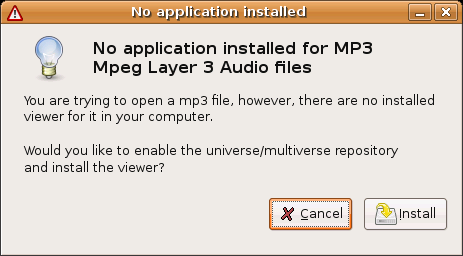
\includegraphics[scale=0.75]{figure/ubuntu_mp3.png}\label{dialog}
	\end{center}
	\caption{\textit{Il primo ``dialog'' per l'installazione del supporto MP3}}
\end{figure}

Questa soluzione, che a livello pratico non richiede particolari competenze informatiche come la capacità di installare il codec MP3 personalmente nel sistema, ha consentito ad Ubuntu di ottenere moltissimi utenti (soprattutto in Europa e negli stati ``liberi'') che non hanno sentito opprimente la copertura brevettuale di altri paesi arrivare fino al proprio.
% \section{Cosa si può fare/non fare in USA in questa circostanza}
% \section{Cosa si può fare/non fare in UE in questa circostanza}

%\include{capitolo5}
%\include{capitolo6}


\appendix

%\include{appendici}

\backmatter
\bibliographystyle{IEEEtran}
\bibliography{bibliografia}
%\include{biblio}

%\printindex % se si fa l'indice analitico.

\end{document}
